\chapter{Probing Star Formation in Clustered environments: the case of IRAS200050+2720 and NGC 2071}

\section{Introduction}
Most stars in the Galaxy form in cluster environments of sizes 2-4 pc, often containing more than 100 young stellar objects (YSOs), with typical separations of $<$0.05~pc between stars near their centers \citep{Porras:2003kxa, Allen:2007wqa, Gutermuth:2009gca}.
Previous studies have been effective in elucidating the young stellar content and distribution in clouds on large scales (parsec down to 0.05~pc) \citep{Evans-ARAA2012}, but young cluster cores, born in dense portions of molecular clouds, are more difficult to observe. They are obscured at optical through near-IR wavelengths. At mid-IR through far-IR wavelengths, the material surrounding YSOs and involved in the stellar birth process emits due to heating by the young stars, but the resolution to date has not been sufficient to isolate individual stars in the cores of most nearby young clusters.

Space telescopes such as \textit{Spitzer} and WISE have tremendous sensitivity, which made them so scientifically productive, but it limits their utility in the densest regions of star-forming clusters because of detector saturated and imaging artifacts (See \citep{2008ApJ...672.1013P} for examples). This is particularly problematic at wavelengths of \SI{24}{\micro\meter} and beyond, where a bright cluster star can dominate a region 3-5 nominal resolution elements out from the star. In fact, it is often difficult for \textit{Spitzer} and WISE to provide good flux estimates for even the brightest YSOs in the cores of clusters.

The FORCAST instrument on SOFIA provides the opportunity to study cluster cores at 10 to \SI{37}{\micro\meter} with better angular resolution than \textit{Spitzer} and WISE, without saturation even on the brightest sources. Although it is less sensitive than space-based instrument at comparable wavelengths due to the large thermal background noise at 13~km altitude, FORCAST images can lift degeneracies in assigning flux by separating sources that were previously unresolved or hidden by saturation artifacts. The mid-infrared fluxes of very clustered objects are essential contraints on their YSO's spectral energy distribution (SED) which is used to determine luminosity and evolutionary state.

This paper presents the results for two clusters, IRAS~200050
and NGC~2071, which were observed as part of a FORCAST survey program to observe bright, nearby star-forming cluster cores for which the \textit{Spitzer} and WISE archival data show extensive amounts of saturation and source confusion based on near infrared images. 

Section 2 provides an overview of what is know about the two clusters. In section 3, we describe our data and reduction methods in detail, and discuss systematic of the FORCAST instrument. Section 4 presents our SOFIA images and discusses them in the context of other observations. Section 5 discusses flux measurements for cluster sources at other wavelengths and outlines our procedures for deriving improved fluxes where applicable. Section 6 presents Spectral Energy Distributions and fits for the SOIFA sources, and section 7 discusses our findings.

\section{Target Clusters}
IRAS~20050+2720 and NGC~2071 are embedded young stellar clusters with total luminosities in the cores that are characteristic of intermediate mass YSOs. The following two subsections provide overviews of each cluster and its environment.

\subsection{IRAS20050+2720}

IRAS~20050+2720 is part of an active site of intermediate-mass star formation in the Cygnus Rift located at 700~pc \citep{Wilking:1989el}, with the particularity that it doesn't seem to contain any massive stars \citep{Gunther:2012dq}. The main cluster core is associated with water and methanol masers \citep{Palla:1991up,Fontani:2010cf} and multipolar molecular outflows observed at millimeter wavelengths \citep{Bachiller:1995cy,Anglada:1998uu,Beltran:2008gu}, suggesting that the region might have experienced a recent episode of star formation in the past 0.1 Myr which contrasts with the average age of the cluster of 1 Myr \citep{Chen:1997tb,Gutermuth:2005hx}. \cite{Gutermuth:2009gca} have identified $>170$ YSOs surrounding the core and measured their continuum fluxes up to \SI{8}{\micro\meter} with IRAC. While measurements at longer wavelengths were able to provide estimates of the total mass of the cluster \citep[e.g. using IRAS,][388~$L_\odot$]{Molinari:1996td}, the measurements are confused in the densest region and it has not been possible to properly associate the far-IR emission with its short wavelength counterpart because of the small separation between IRAC-detected protostars. The IRAS point source was classified as a luminous class 0 protostar \citep{Bachiller:1996ja}, and its emission associated with the bright millimeter source MMS1 to the northwest of the core \citep{Chini:2001fa}. \cite{Beltran:2008gu} show strong evidence that this region has multiple generations of stars, and suggest that a group of low-mass stars first completed its main accretion phase, before setting the stage for the birth of new intermediate-mass stars at the core of this cluster.

We have observed two fields within the cluster (see Fig.~\ref{fig:IRAS20050_RGB}), including the brightest core at $20^h 07^m 06.70^s +27^{\circ} 28'54.5''$. Multiple sources in the core can be distinguished in the IRAC maps, but the core appears extended in Spitzer MIPS at \SI{24}{\micro\meter}, and is identified as a single source with WISE. No good high resolution far-infrared continuum data longward of \SI{24}{\micro\meter} was available for this source.

%Cite also: \citep{Kumar:2006jo} if we want to talk about multiple generations of star formation.

\begin{figure*}
\begin{center}
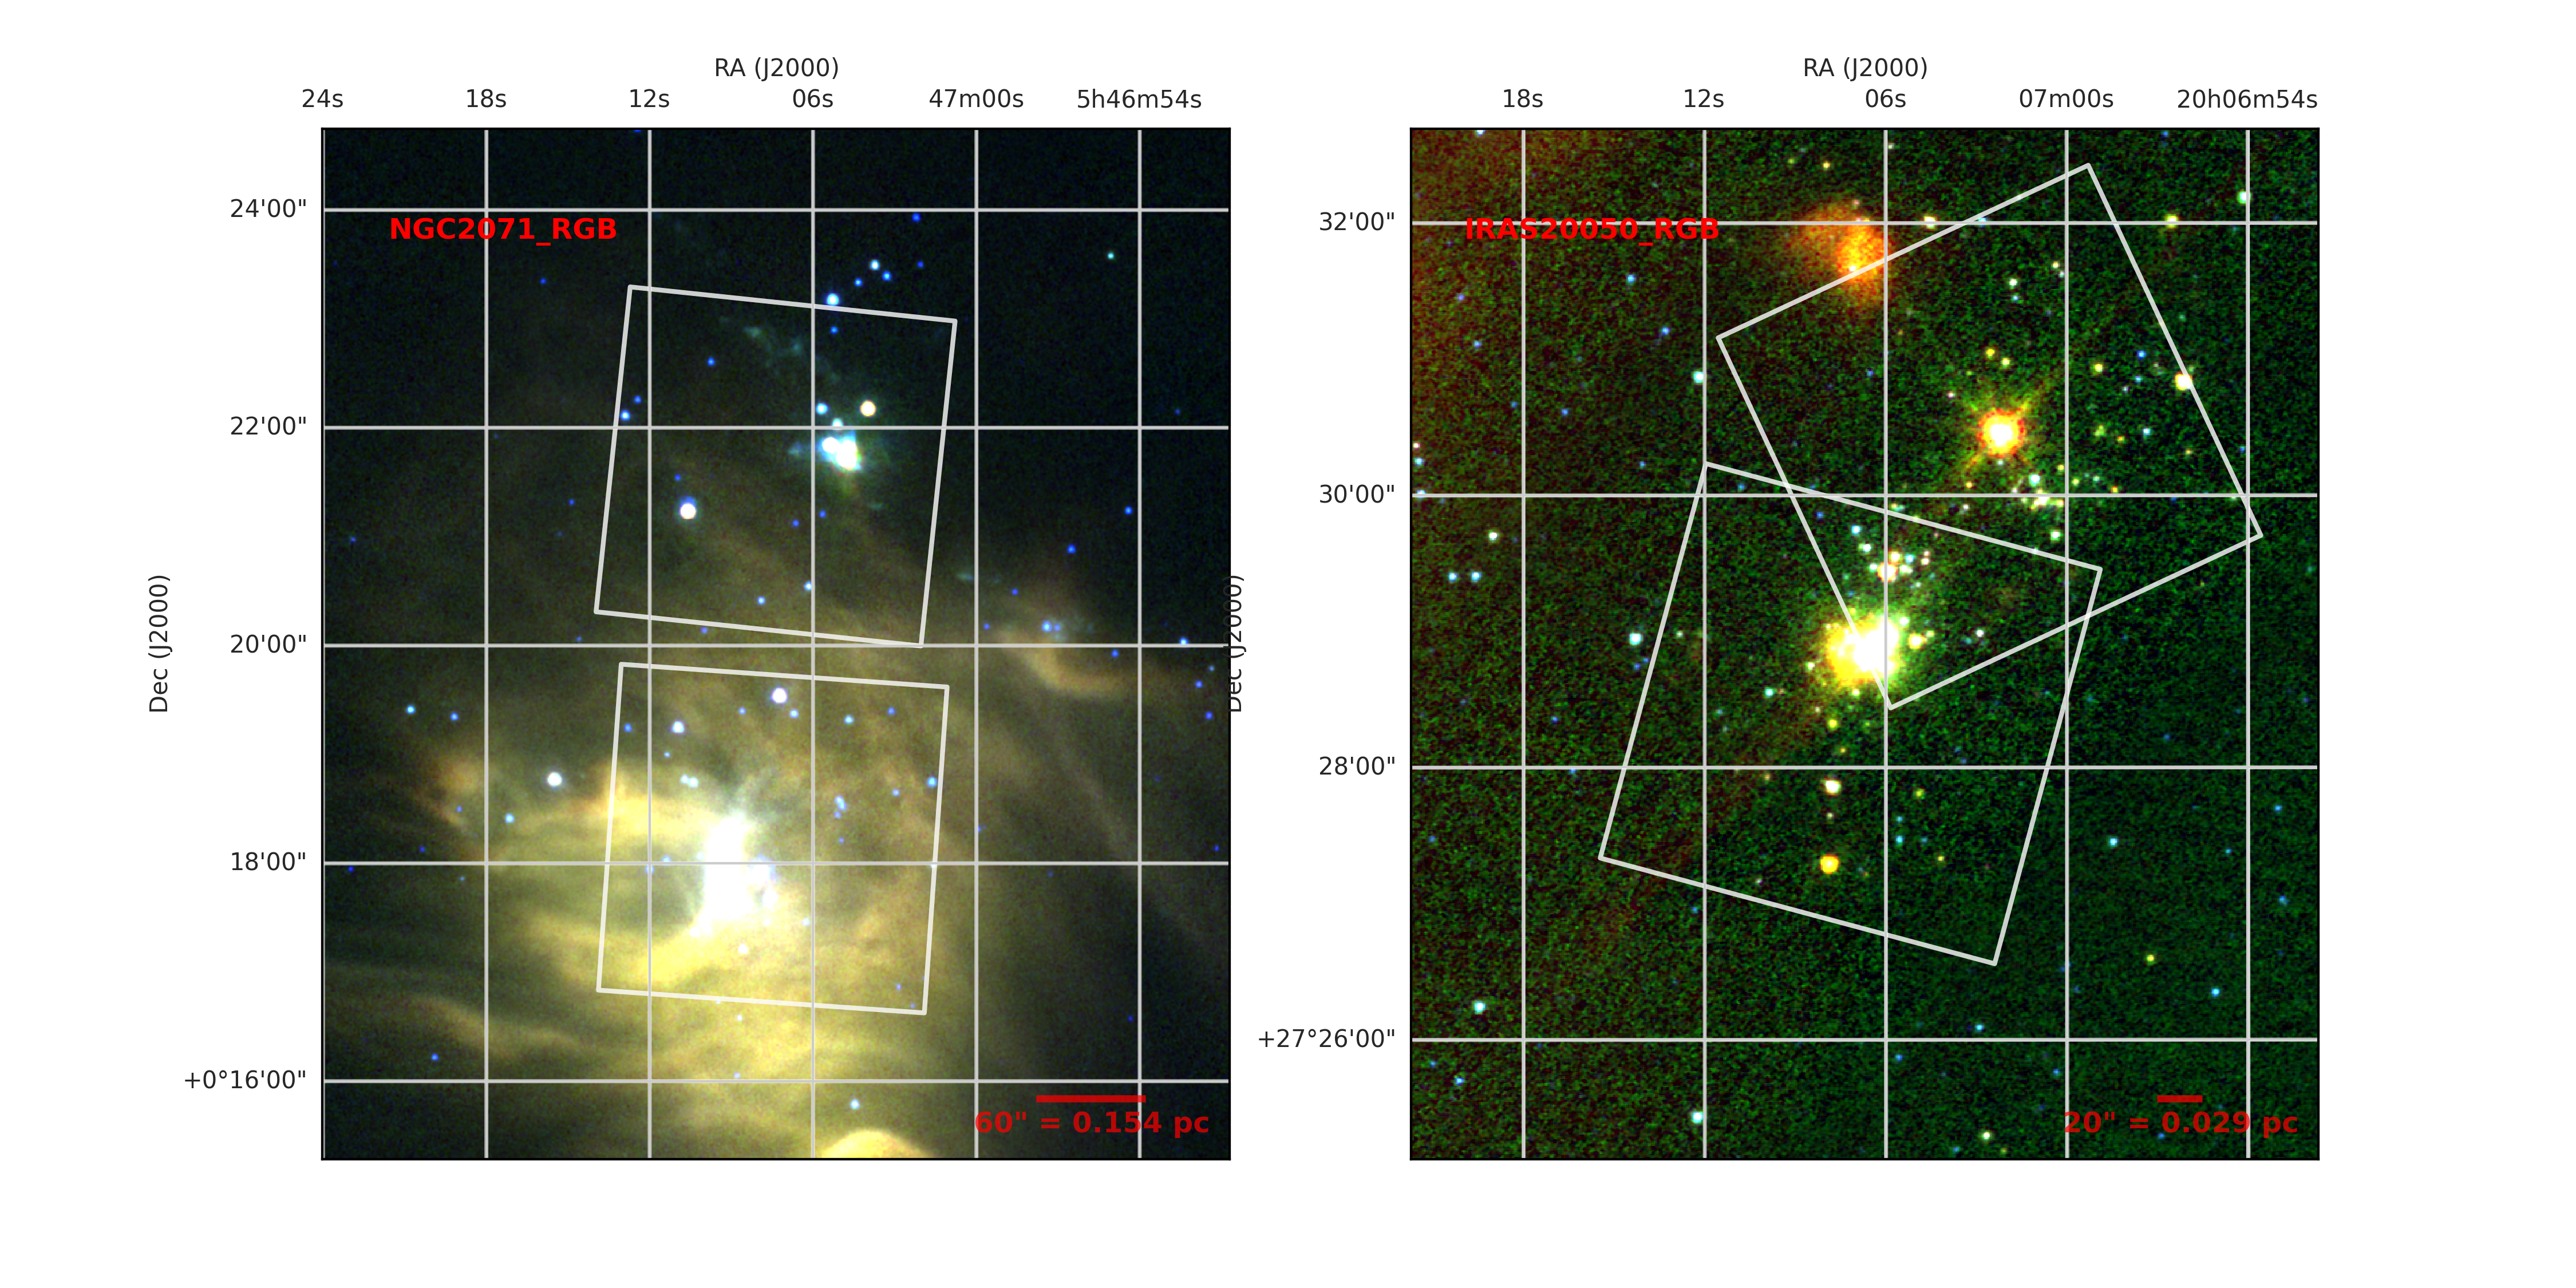
\includegraphics[width=\textwidth]{Figures/RGB.png}
\label{fig:RGB}
\caption{
%\textit{Left:} The two white squares correspond to the FORCAST fields that we observed in around the core of IRAS~20050+2720. The background RGB image is a composition of \textit{Spitzer} IRAC 8~$\um$ (red), \textit{Spitzer} IRAC 5.7 $\um$ (green) , and IRAC 3.6~$\um$ (blue). The dashed red square at the center of the image correspond to the core of the cluster, displayed in greater detail in  the picture to the right. \textit{Right:} This RGB picture shows the IRAC 1, 3, and 4 bands of the core at the center of Fig.~\ref{fig:IRAS20050_RGB}. The white contours represent the contours of the FORCAST 37~$\um$ maps, and the red circles show the FORCAST-identified point sources. An infrared nebulosity can be seen to the East of the core with physical projected size of about 0.015~pc, surrounding a cavity with slightly smaller size. The nebulosity and its cavity can be seen all the way up to 37~$\um$. The far-IR emission is mapped well onto the IRAC sources, except for SOF4, for which almost no emission can be seen at shorter wavelengths. SOF4 matches the location of the bright millimeter source MMS1 \citep{Chini:2001fa}.}
}
\end{center}
\end{figure*}

% \begin{figure*}
% \begin{center}
% \includegraphics[width=5in]{}
% \label{fig:IRAS20050_RGB_core}
% \caption{}
% \end{center}
% \end{figure*}


[Include a discussion about de-reddening towards that region?]

\subsection{NGC 2071}
The NGC~2071 star-forming region is one of several active areas of star formation in the northern part of L1630 giant molecular cloud which is located at a distance of 390 pc \citep{A-T1982}. 
NGC~2071 itself is a reflection nebula.
The NGC~2071 infrared cluster, located about 4' north of the reflection nebula, is a region of intermediate mass star formation \citep{Strom1976, Persson1981, Butner1990}. Maps of the cloud in CO and its isotopomers \citep{Buckle2010} show a large scale clump with $\sim$1,000 M$_\odot$ associated with the cluster. Dust continuum emission at $\lambda$=0.85 and 1.3 mm peaks on center of the cluster extending ~1' in diameter containing ~30 M$_\odot$ of gas and dust \citep{Johnstone2001,Mitchell2001,Launhardt1996}. Emission from CS in the J=2-1 through J=7-6 indicate that the gas in this region is centrally condensed with a density of ~10$^6$ cm$^{-3}$ \citep{Zhou1990}. 

There are a number of near infrared surveys of the young cluster \citep[e.g.,][]{Strom1976,Lada1991,Megeath2012,Spezzi2015}. \cite{Spezzi2015} identify 52 YSOs associated with the NGC~2071 cluster, with the majority Class II sources. \cite{Flaherty2008} estimate an age of $\sim$2 Myr for the cluster, consistent with the large fraction of Class II sources (\cite{Evans2009}. The brightest far infrared emission from the cluster is associated with the IRS1 region \citep{Harvey1979,Butner1990}, which has an estimated total luminosity of 520~L$_\odot$. The immediate region of IRS 1 is, in fact, home to a number of YSOs that are infrared, X-ray, and radio sources \citep{Skinner2009,C-G2012,Kempen2012}. The radio \citep{C-G2012} and H$_2$ emission line imaging indicate that IRS~1, IRS~2, IRS~3, and, perhaps, VLA~1 are YSOs with outflows. The larger scale molecular outflow associated with this region is well studied in a number of molecules \citep{Bally1982,Chernin1993,Stoji2008}.
\begin{figure*}
\begin{center}
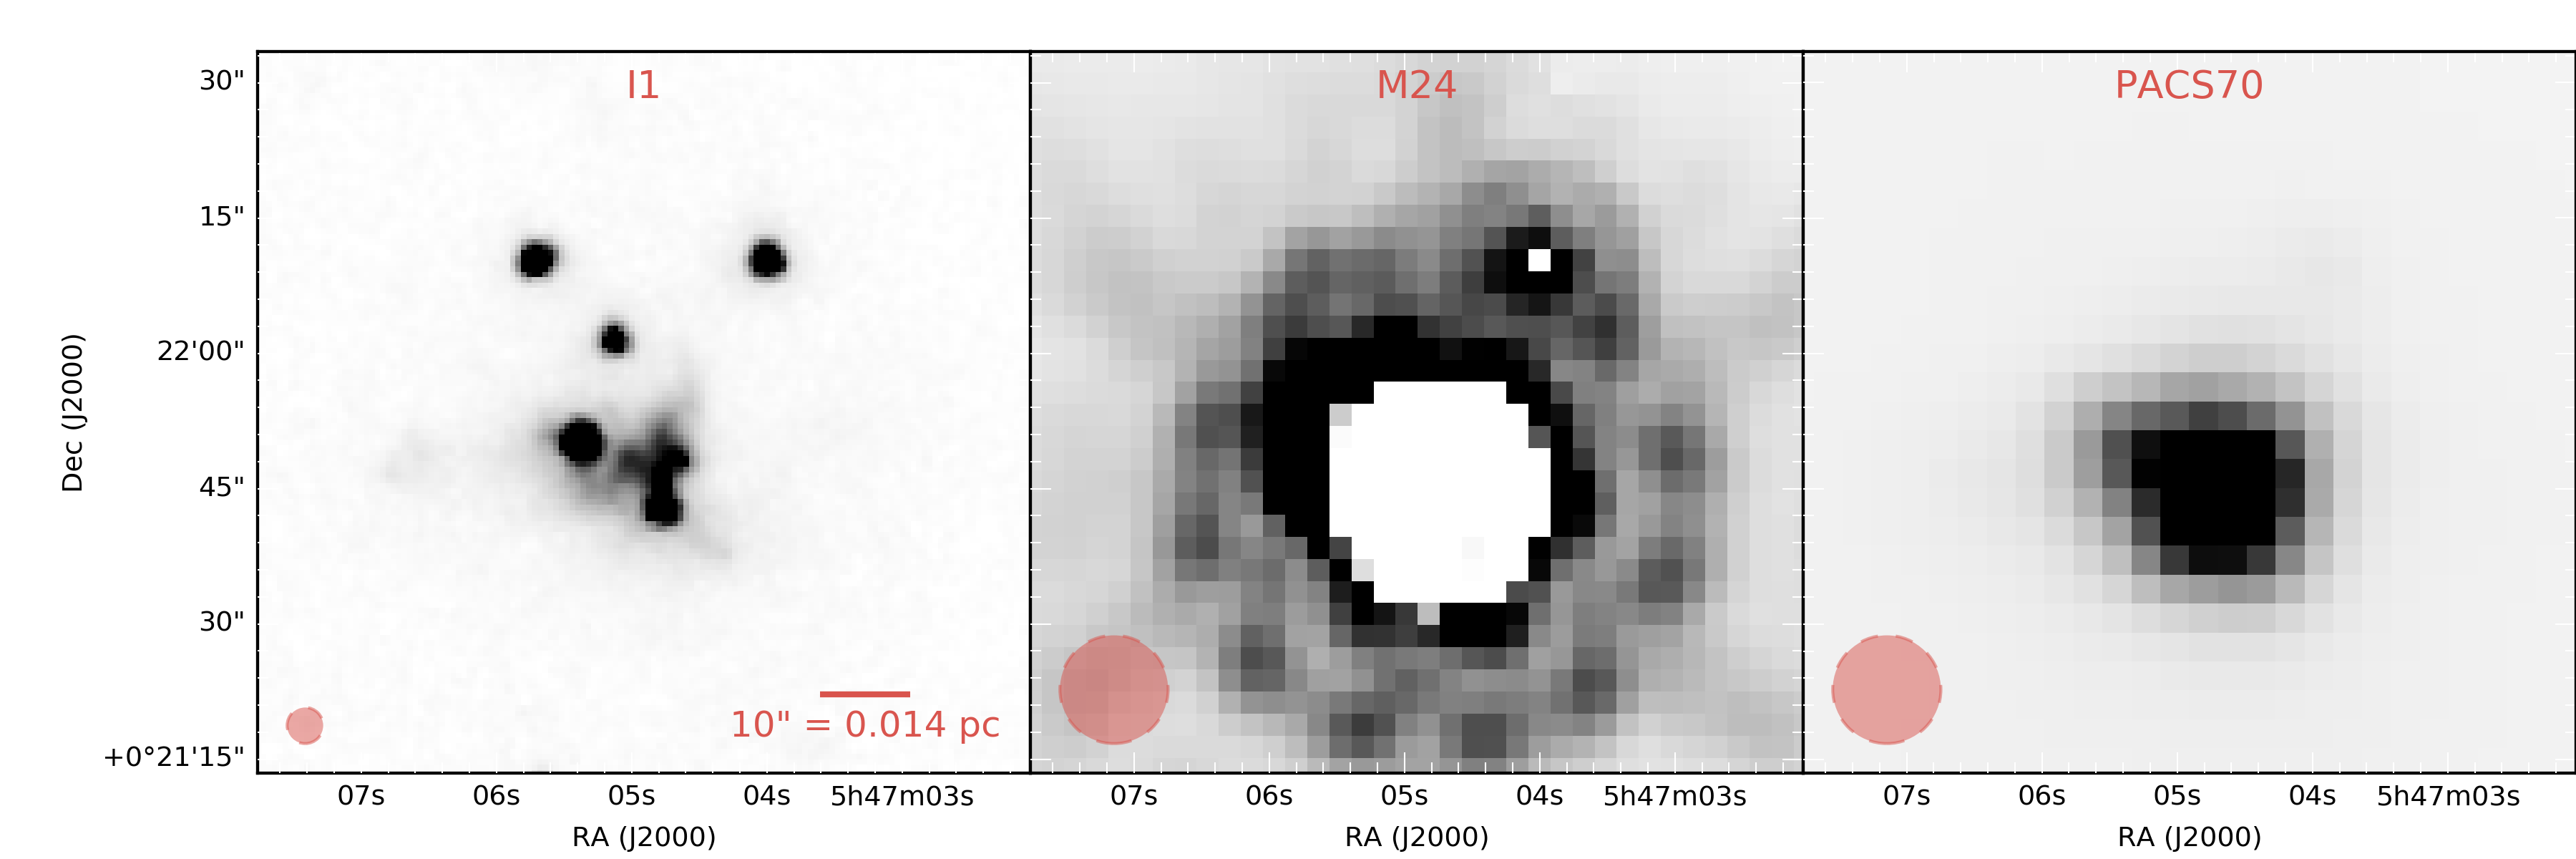
\includegraphics[width=\textwidth]{Figures/NGC2071_saturated_mosaic.png}
\label{fig:n2071saturated}
\caption{%NGC 2071 IRS~1 Region: The left panel show the Spitzer IRAC 3.1~$\um$ image. The right panel is the Herschel 70~$\um$ image. The green plus marks indicate the positions of IRS~1, IRS~2, IRS~3, and VLA~1. The inner red circle show the extend of the saturated region in the Spitzer MIPS 24~$\um$ image and the outer red circle encompasses the region strong affected by imaging artifacts. The gray circle on the lower right of the right panel is the resolution the 70~$\um$ image.
NGC2071 seen with IRAC, MIPS and Herschel.}
\end{center}
\end{figure*}

Figure \ref{fig:n2071overview} shows the Spitzer 3.1~$\mu$m image of the IRS~1 region on the left \citep[image from Spitzer Archive:][]{Megeath2012} and the Herschel 70~$\mu$m image on the right (image from Herschel Archive: Gould Belt Project, P.I. Andr\'e). The plus marks in both panels indicate the position of the brighter YSOs: IRS~1, IRS~2, IRS~3, IRS~4, and VLA~1. The inner red circle with a diameter of 26" indicates the extend of the saturated region in the Spitzer MIPS 24~$\mu$m image; the outer red circle, diameter 60", encompasses the region with strong imaging artifacts in the MIPS 24~$\mu$m image.
The right panel shows Herschel 70~$\mu$m image which does not resolve the emission from IRS~1, IRS~2, IRS~3, and VLA~1. The centroid of the 24~$\mu$m and 70~$\mu$m emission is between IRS~1 and VLA~1 indicating that several of the sources are contributing to the total observed emission. Interferometric observations show that the millimeter wavelength dust emission is dominated by envelopes associated with IRS~1 and IRS~3, with estimated masses of 8.2 and 12.3~M$_\odot$ material, respectively \citep{Kempen2012}. The millimeter emission also reveals the presence of disks with radii $\le$100~AU associated with IRS~1 and IRS~3 \citep{Kempen2012}.

The luminosities and masses of the individual source, IRS~1, IRS~2, IRS~3, and VLA~1, are not known. The Spectral Energy Distributions (SEDs) shortward of 10~$\mu$m support their identification as embedded YSOS \citep{Skinner2009}. \cite{Skinner2009} gives a clear discussion of the possibilities for IRS~1 and concludes that it is likely a mid-to late B~star. \cite{Kempen2012} find luminosities of 10, 3.4, and $\le$27~L$_\odot$ for IRS~1, 2, and 3, respectively, and stellar masses of $\le$1~M$_\odot$ for each, based on SED fitting. These masses and luminosities are not consistent with estimate of the total luminosity of the region of 520~L$_\odot$ \citep{Butner1990}. The far infrared images from Herschel reveal that IRS~1 alone does not totally dominate, as seen in Figure N; IRS~1, VLA~1, and IRS~3 likely make substantial contributions to the emission with lesser emission from IRS~2 and IRS~4.

\section{SOFIA Observations}
NGC 2071 and IRAS 200050+2720 were observed with the FORCAST instrument on SOFIA as part of a survey of selected nearby ($\le$1~kpc) bright star-forming clusters which show high protostellar density \citep{Gutermuth:2009gca} and are located in the northern hemisphere. The survey focussed on the clusters that contain one or more saturated or confused region in the archival \textit{Spitzer} and WISE data.

\subsection{Data Acquisition}
The IRAS 200050 and NGC~2071 observations were collected over three flights out of the 10-flight survey campaign. A summary is shown in Table~\ref{tab:obssummary}. Because the clusters are dominated by bright sources, the observations fit into small flight segments which filled gaps in the flight schedule. The source coordinate in Table~\ref{tab:obssummary} correspond to the centers of the green areas in Fig.~\ref{fig:IRAS20050_RGB} and Fig.~\ref{fig:n2071overview}. In each cluster, two fields separated by $\sim$ 3 arcminutes were observed to focus on two saturated regions. All fields were observed using the chop-and-node C2N mode from FORCAST, with 9-point dithering to reduce the flat field issues.

%\capstartfalse
%\begin{deluxetable*}{ccccccccccc}
%\tablecaption{target list}
%\tablenum{1}
%\tablehead{\colhead{Cluster} & \colhead{RA} & \colhead{DEC} &  \colhead{Flight} & \colhead{Fields} & \colhead{Dist.} & \colhead{Time/Field} & \colhead{Sen{\_}11} & \colhead{Sen${\_}$19} & \colhead{Sen${\_}$31} & \colhead{Sen${\_}$37} \\
%\colhead{} & \colhead{(deg)} & \colhead{(deg)} & \colhead{} & \colhead{}  & \colhead{(pc)} & \colhead{(s)} & \colhead{(Jy)} & \colhead{(Jy)} & \colhead{(Jy)} & \colhead{(Jy)}} 
%\startdata
%IRAS20050+2720 & 301.771 & 27.481 & F166, F131 & 2 & 700$^{1}$ & 253 & 0.026 & 0.039 & 0.068 & 0.127 \\
%NGC2071 & 86.775 & 0.363 & F192 & 2 & 420$^{2}$ & 35 & 0.118 & 0.119 & 0.196 & 0.474
%\enddata
%\label{tab:obssummary}
%\end{deluxetable*}
%\capstarttrue 


We observed the clusters in 4 bands: 11.1, 19.7, 31.5 and \SI{37.1}{\micro\meter}. The requested observation time in each band was calculated to detect YSOs with rising spectral energy distribution (SED) of same luminosity at the two distances of the clusters. We estimated integration time based on a rising-SED protostar model for $\sim 1.5\Lsun$. [HOW SHOULD I JUSTIFY THE FLUXES THAT WE SET AS OUR LIMITS?]

Average observing time per field and average measured 1-sigma sensitivity levels are shown in Table~\ref{tab:obssummary} for the 4 bands. The measured background levels indicate the smallest detectable point source flux density at each wavelength, based on the noise measurements in the image itself. Bands 11.1 and \SI{37.1}{\micro\meter} were observed simultaneously using a dichroic filter, as were 19.7 and 31.5. However, in order to reach the required flux sensitivity for the \SI{37.1}{\micro\meter} band, we completed some of our observations with single-band observations at \SI{37.1}{\micro\meter}. 

% \begin{longtable*}{ccccccc}
% \hline
% \hline
% Cluster Name & Field & Field Coordinates & Band & Time (s) & Flight & Date \\
% \hline

% IRAS20050+2720 & 2 & 20h07m03s +27d30m38s & 11.1d & 135 & F131 & 2013-09-17 \\
% IRAS20050+2720 & 2 & 20h07m03s +27d30m30s & 19.7d & 140 & F166 & 2014-05-02 \\
% IRAS20050+2720 & 2 & 20h07m03s +27d30m47s & 31.5d & 160 & F166 & 2014-05-02 \\
% IRAS20050+2720 & 2 & 20h07m04s +27d31m02s & 37.1d & 135 & F131 & 2013-09-17 \\
% IRAS20050+2720 & 3 & 20h07m06s +27d28m12s & 11.1d & 135 & F166 & 2014-05-02 \\
% IRAS20050+2720 & 3 & 20h07m06s +27d28m05s & 19.7d & 84 & F166 & 2014-05-02 \\
% IRAS20050+2720 & 3 & 20h07m06s +27d28m13s & 31.5d & 96 & F166 & 2014-05-02 \\
% IRAS20050+2720 & 3 & 20h07m06s +27d28m06s & 37.1d & 126 & F166 & 2014-05-02 \\
% \hline

% NGC2071 & 1 & 05h47m07s +00d17m49s & 11.1d & 18 & F192 & 2015-02-05 \\
% NGC2071 & 1 & 05h47m07s +00d18m02s & 19.7d & 11 & F192 & 2015-02-05 \\
% NGC2071 & 1 & 05h47m06s +00d17m55s & 31.5d & 11 & F192 & 2015-02-05 \\
% NGC2071 & 1 & 05h47m07s +00d18m03s & 37.1d & 21 & F192 & 2015-02-05 \\
% NGC2071 & 2 & 05h47m07s +00d21m30s & 11.1d & 18 & F192 & 2015-02-05 \\
% NGC2071 & 2 & 05h47m07s +00d21m31s & 19.7d & 18 & F192 & 2015-02-05 \\
% NGC2071 & 2 & 05h47m07s +00d21m34s & 31.5d & 24 & F192 & 2015-02-05 \\
% NGC2071 & 2 & 05h47m07s +00d21m34s & 37.1d & 21 & F192 & 2015-02-05 \\

% \caption{List of observations}
% \end{longtable*}

%Make sure to mention the distances picked and the references for it, as well as the cluster's age estimate
%Need to find references to cite for details about each region
\subsection{Data reduction}
The data are processed through various versions of the online pipeline to yield Level 2 data products available on the archive \citep{Herter:2013by}. We apply our own reduction procedure and photometry pipeline on those products to derive final images, source positions, fluxes and sensitivities. The software utilizes the Python \textit{astropy} package \citep{2013A&A...558A..33A} and its associated modules \textit{photutils} and \textit{APLpy}. 

\subsubsection{Pre-treatment}
Some manual treatment of each image is necessary before it can be analyzed by our software, which follows this procedure: a) visually aligning the WCS coordinate system, often 10-20" off, using point sources and archival data from other wavelengths and facilities such as IRAC \SI{8}{\micro\meter}; b) cropping the images to clean off the nodded fields, and c) identify the coordinates of each source, both point-like and extended.

After these manual steps, the Level 2 images are multiplied by the calibration factor provided by the online pipeline, which converts them to Jy/pixel. We do not proceed to any systematic color correction, but the effects on the fluxes are very small \citep{Herter:2013by}.
\begin{comment}
\begin{enumerate}
\item Adjust WCS coordinates: use images at other wavelengths (2MASS, IRAC, MIPS, WISE) to re-align the (RA, DEC) position of the field. We estimate that this process is good to within one SOFIA pixel (0.768") for the fields where one or more point sources can be identified. Extended fields are less trustworthy, since matching the extended emission to other wavelengths is harder. The rotation of the field produced by the SOFIA pipeline is correct for all of our data. 
\item Crop each image, remove chopped fields, remove artifacts.
\item Identify and categorize sources: isolated point sources, clustered point sources, and extended sources. For extended sources, a circular or elliptical aperture is used to try to encompass the entirety of the emission.
\item Manually identify a location in the field that corresponds to a representative background.
\end{enumerate}
\end{comment}
\subsubsection{Source flux extraction and calibration}
\begin{comment}
We feed the adjusted FITS and associated metadata files to a photometry pipeline. The pipeline first processes all the calibrator stars that are observed during each flight, with each filter setting, and derives a new aperture correction factor for each image, based on an aperture of 4 pixels radius (3.072") and an aperture of 12 pixels radius. We consider that the latter aperture contains all the flux from a given point source.

We distinguish between 3 types of sources after manual identification: \textit{isolated}, which are point sources with no nearby objects; \textit{clustered}, which are point sources with nearby objects; and \textit{extended}, which are not consistent with being point sources. [THIS PARAGRAPH MAY GO AWAY IF WE DON'T WANT TO TALK ABOUT GENERALITIES ABOUT THE PIPELINE]


For point sources, we use our standard aperture of 4 pixels at all wavelengths. We consider an annulus surrounding the source extending from 12 to 20 pixels radius (24 to 40 for clustered sources): the local background is determined from the mode of the pixels in the annulus, while the sensitivity is calculated by measuring the standard deviation of 4-pixel apertures within that annulus [Cite Taro's paper and the Herschel photometry paper that Tracy gave us]. We apply the aperture correction derived from the calibrator observations taking during that flight.

For extended sources, an elliptical aperture is determined manually from the \SI{37}{\micro\meter} images. The local background is determined from the mode of an elliptical annulus, with an inner boundary at the elliptical aperture and an outer boundary corresponding to an ellipse 20\% larger. The sensitivity quoted is the point source sensitivity, and is determined following the same method as for point sources, using the standard deviation of apertures spread across the elliptical annulus. [NO NEED TO MENTION THIS SINCE WE MIGHT NOT TREAT EXTENDED SOURCES]

The photometry from sources that were observed in different flights is then combined to increase the signal-to-noise ratio. This combination takes into account the sensitivity of each source by appropriately weighing each image.

Although we can compute source sensitivities based on the local noise, and we use the calibrators each flight to determine the aperture correction, observations with SOFIA have additional noise from the water vapor overburden and air mass, as well as from the flat field variations. These noise contributions usually amount to much higher than the sensitivities estimated from the local background, and we follow the recommendation from \citep{Herter:2012hv} to adopt a 20\% uncertainty for our flux estimates. 

\end{comment}

\subsection{Photometry at other wavelengths}

\subsection{Instrumental Characterization}
[THIS WHOLE DISCUSSION MIGHT FIT BETTER IN THE PAPER ABOUT THE WHOLE SURVEY, RATHER THAN THIS PAPER WHICH IS JUST ABOUT TWO CLUSTERS...]
The three flights discussed here were part of the total of 10 data flights for the entire survey. The larger context of the entire survey allowed us to follow the evolution of the instrument properties throughout the two years of science observations. We discuss three metrics: the evolution of the aperture correction factor, the evolution of the instrument's residuals, and the evolution of the PSF size, through half width at half max of the encircled energy distribution, that we call $\Rfifty$. This is done in an attempt to assess the uncertainties in our flux determination, and our confidence in determining that sources are point-like or extended. %This study is based  on the large number of calibrator observations during our 10 science flights.

\subsubsection{PSF size}

Fig~\ref{fig:average_EE} shows the average of the normalized encircled energy distribution of the PSF, measured on all the calibrators of our sample. Each curve represents one of the five different combinations of bandpass filter and dichroic setting that we use for our observations: \SI{11.1}{\micro\meter}, \SI{19.7}{\micro\meter}, \SI{31.5}{\micro\meter}, \SI{37.1}{\micro\meter} with dichroic and \SI{37.1}{\micro\meter} without a dichroic (open). 

As expected, the PSF at \SI{37.1}{\micro\meter} is larger than the PSFs at shorter wavelengths, but less that the traditional diffraction limit rule. This indicates that additional PSF smearing is occurring at short wavelengths, likely due to plane jitter and pointing errors. This was predicted and mentioned in the SOFIA Observer's Handbook. Throughout all the flights, the largest 1-sigma error occurs for the \SI{37}{\micro\meter} observations at about XX\%. CONCLUDE ON OUR ABILITY TO DETERMINE WHETHER A SOURCE IS EXTENDED OR NOT.

To look at the behavior of the PSF in more detail, we can use the half width at half maximum of the encircled energy distribution, $\Rfifty$ as a proxy for PSF size. The variation of this quantity for the various flights, bandpass/dichroic setting, and calibrators used is showed in Fig~\ref{fig:Rfifty_dist}. This shows the flight-to-flight differences and, for some calibrators, the in-flight variability. We find that the latter is usually NN\% or less, except for the SOFIA flight on 05-02-2014, for which the spread is quite considerable. The variation from flight to flight is larger than the variation within a given flight, which indicates variability in the observing conditions, systematics, or thermal radiation environment of the observatory between different flights. Hence, we conclude that the extension of a source can be best determined by comparing $\Rfifty$ for that source with $\Rfifty$ for the corresponding calibrator measurement for that flight and dichroic setting, to within NN\%, 1-sigma confidence.
\begin{figure}
\begin{center}

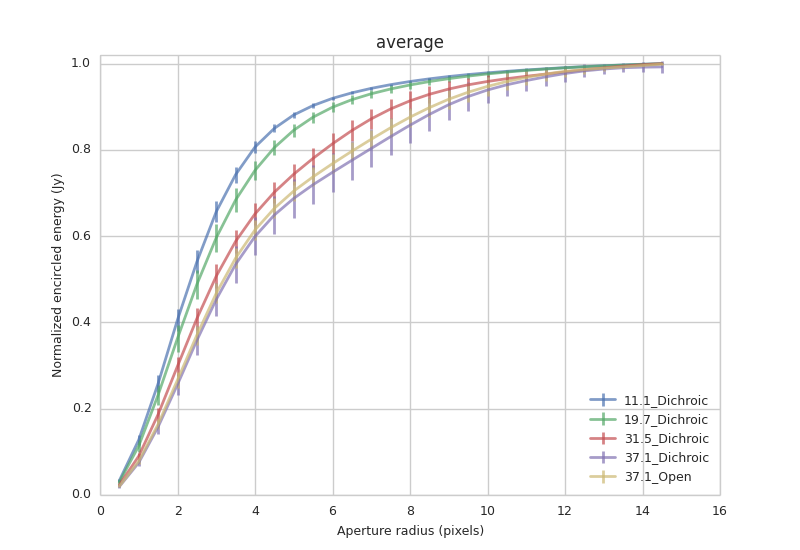
\includegraphics[width=0.45\textwidth]{Figures/average.png}
\label{fig:average_EE}
\caption{PSF size distribution}
\end{center}
\end{figure}

\begin{figure}
\begin{center}

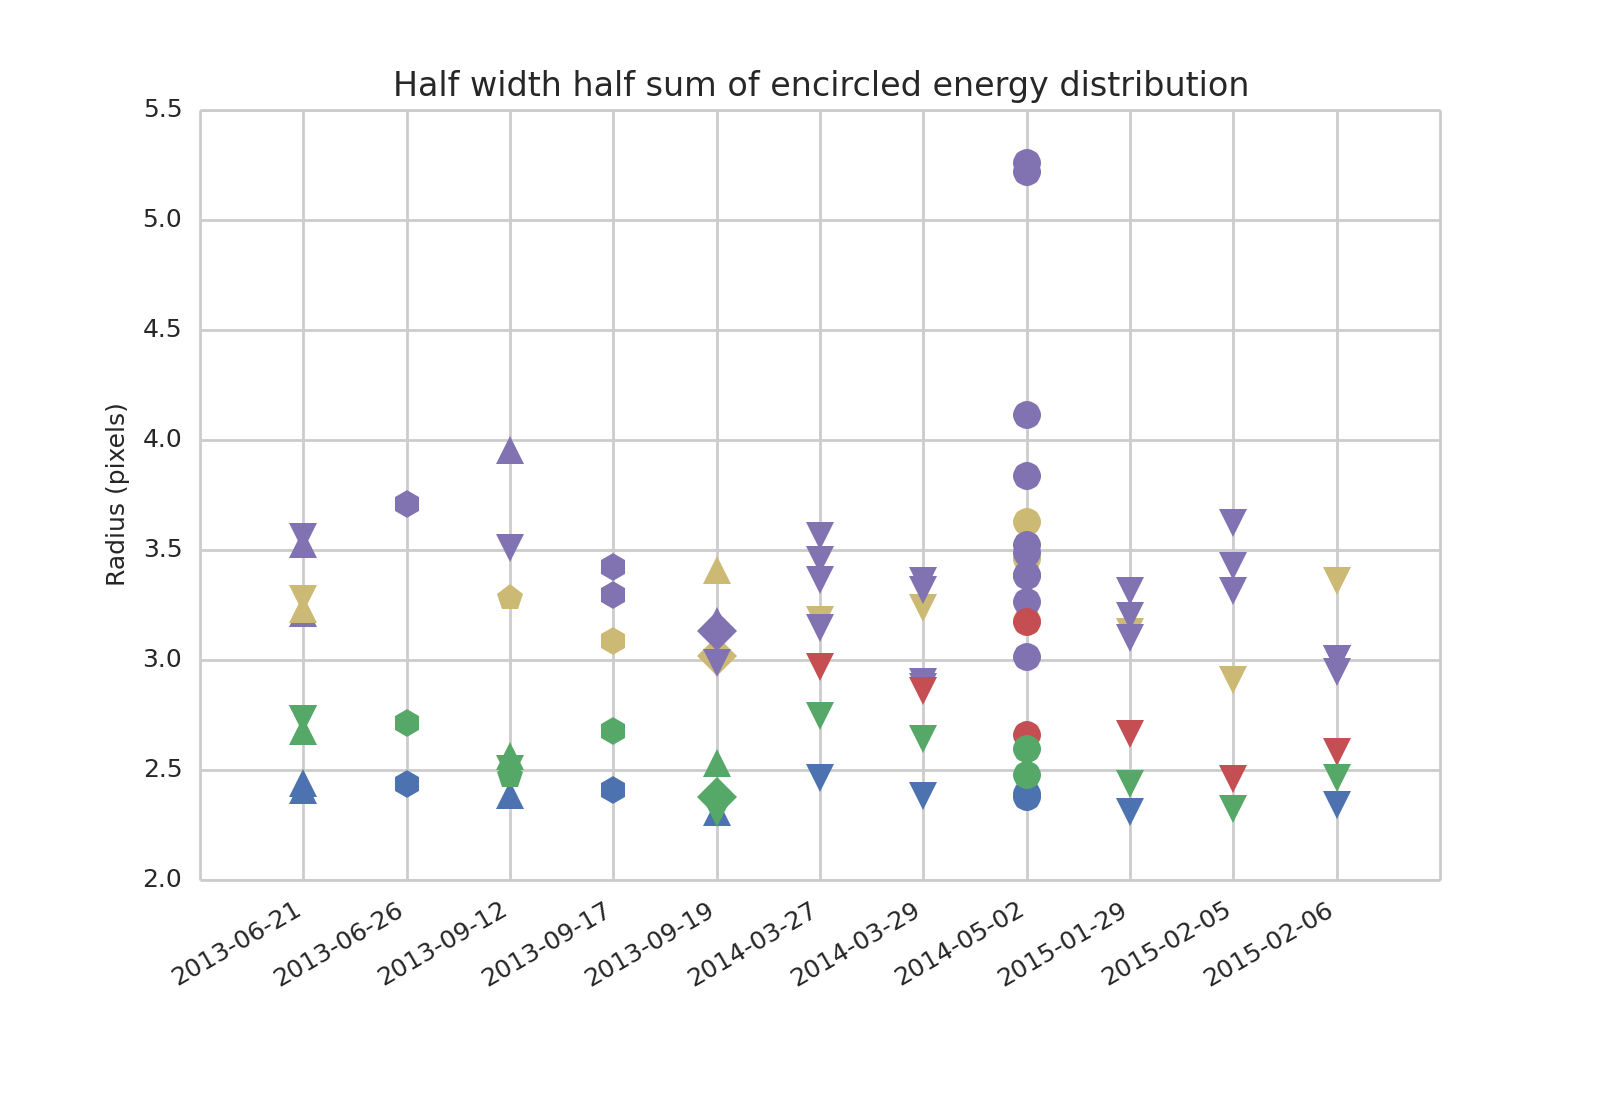
\includegraphics[width=0.45\textwidth]{Figures/fwhs.png}
\label{fig:Rfifty_dist}

\caption{PSF size distribution}
\end{center}
\end{figure}

\subsubsection{Aperture correction}
In Fig~\ref{fig:response}, we plot the aperture correction factor that we compute from the ratio of the flux measured within an aperture of 4 pixels, divided by the flux measured in an aperture of 12 pixel radius, which we consider to be encompassing the total flux in the source. Not surprisingly, this graph follows very closely the plot of $\Rfifty$ shown in Fig~\ref{fig:Rfifty_dist}, showing the close link between the aperture correction factor and the shape of the calibrator's PSF. For the aperture correction variability, we adopt a XX, 1-sigma uncertainty value on the flux estimate.



\subsubsection{Instrument response}
To further study the variability of the observing, we can look at the detector response and the aperture correction evolution after applying the calibration factor. In the ideal conditions, the calibration factor always leads to the same flux measurement of the calibrator source, within the pipeline's systematic errors and residual noise. The detector response is measured here by simply applying aperture photometry on the calibrators to measure their fluxes, using the same local background subtraction as the one described in the previous sections. Calibrator stars are good ways to correct for telescope and atmospheric variability, as their far-infrared fluxes are not expected to vary significantly over any relevant timescale. %We adopt a value of XX, 1-sigma value for the response variability, effectively representing the uncertainties in the observatory and the atmosphere.
In Fig~\ref{fig:response}, we plot all the measured fluxes of the calibrators. The flux variability from flight to flight for a given calibrator is small (typically [CALCULATE THIS]), and the variability within the same flight is even smaller [QUANTIFY]. We adopt a XX, 1-sigma uncertainty value for the absolute flux measurement. This is the residual uncertainty after applying the systematic correction produced by the SOFIA FORCAST online pipeline.



\begin{figure}
\begin{center}

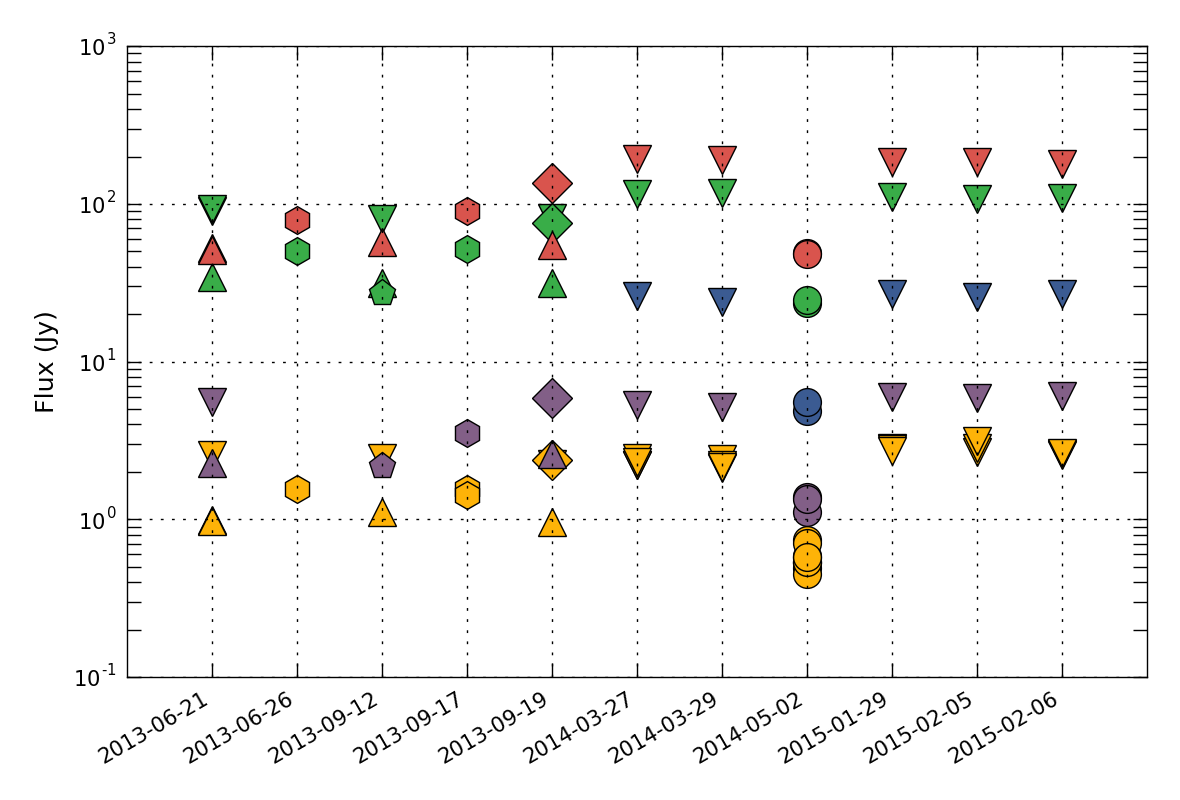
\includegraphics[width=0.45\textwidth]{Figures/Phot_val.png}
\label{fig:response}
\caption{Instrumental response and aperture correction}

\end{center}
\end{figure}

\begin{figure}
\begin{center}
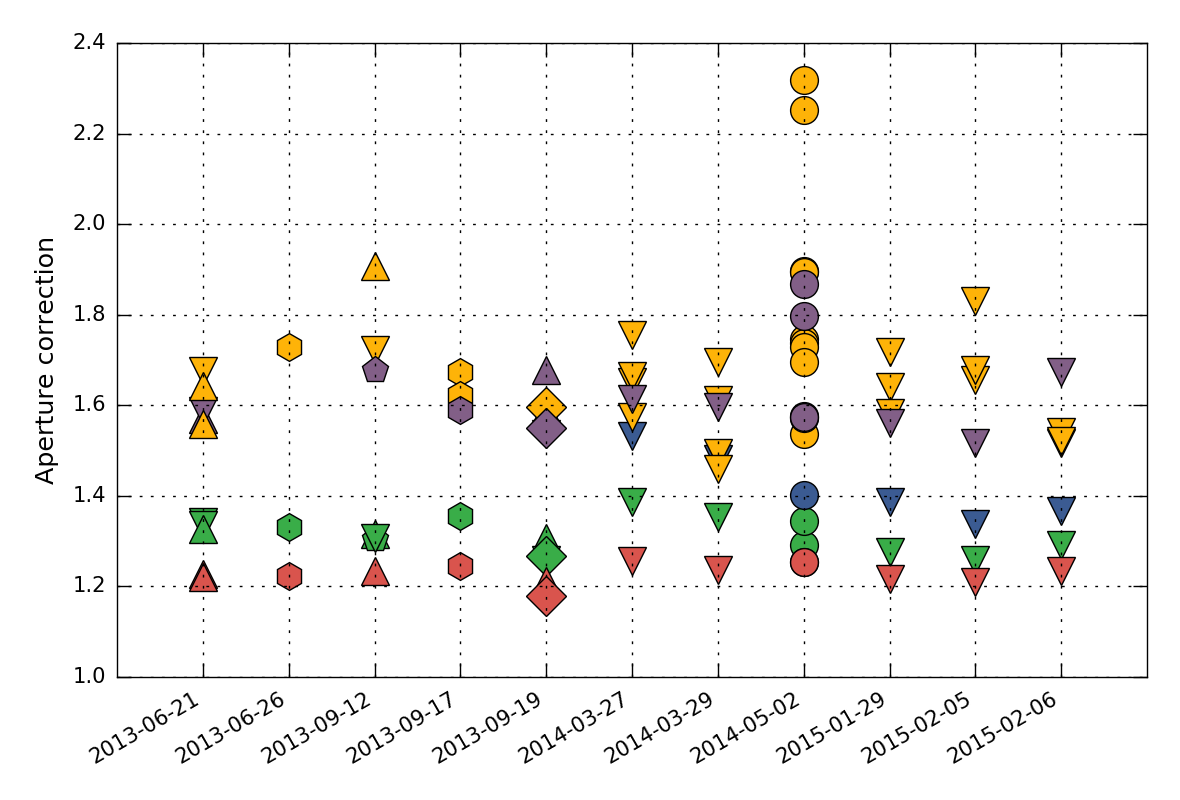
\includegraphics[width=0.45\textwidth]{Figures/Aper_corr.png}
\label{fig:aper_corr}

\caption{Instrumental response and aperture correction}
\end{center}
\end{figure}

%WHAT IS THE BOTTOM LINE FROM THIS DISCUSSION? IS A FLUX MEASUUREMENT LIMITED BY VARIATIONS IN THE PSF IF IT IS BRIGHT? SOMETHING ELSE? IT SEEMS LIKE THE CONCLUSION FROM THIS SECTION SHOULD BE A STATEMENT ABOUT THE SYSTEMATIC ERRORS ON ANY QUOTED FLUX MEASUREMENT AND A STATEMENT ABOUT LIMITATIONS ON KNOWING WHETHER A SOURCE IS EXTENDED RELATIVE TO A POINT SOURCE.
\section{Observational results}
\subsection{IRAS 200050}

SOFIA photometry results, IRAC photometry issues and results; looking at the sources that are fit by guthermuth, we find a 10\% agreement between our photometry results and theirs.

\subsubsection{Photometry results and maps}

\subsubsection{SEDs}


\subsubsection{Upper limits on other sources in the field}

\begin{figure}
\begin{center}
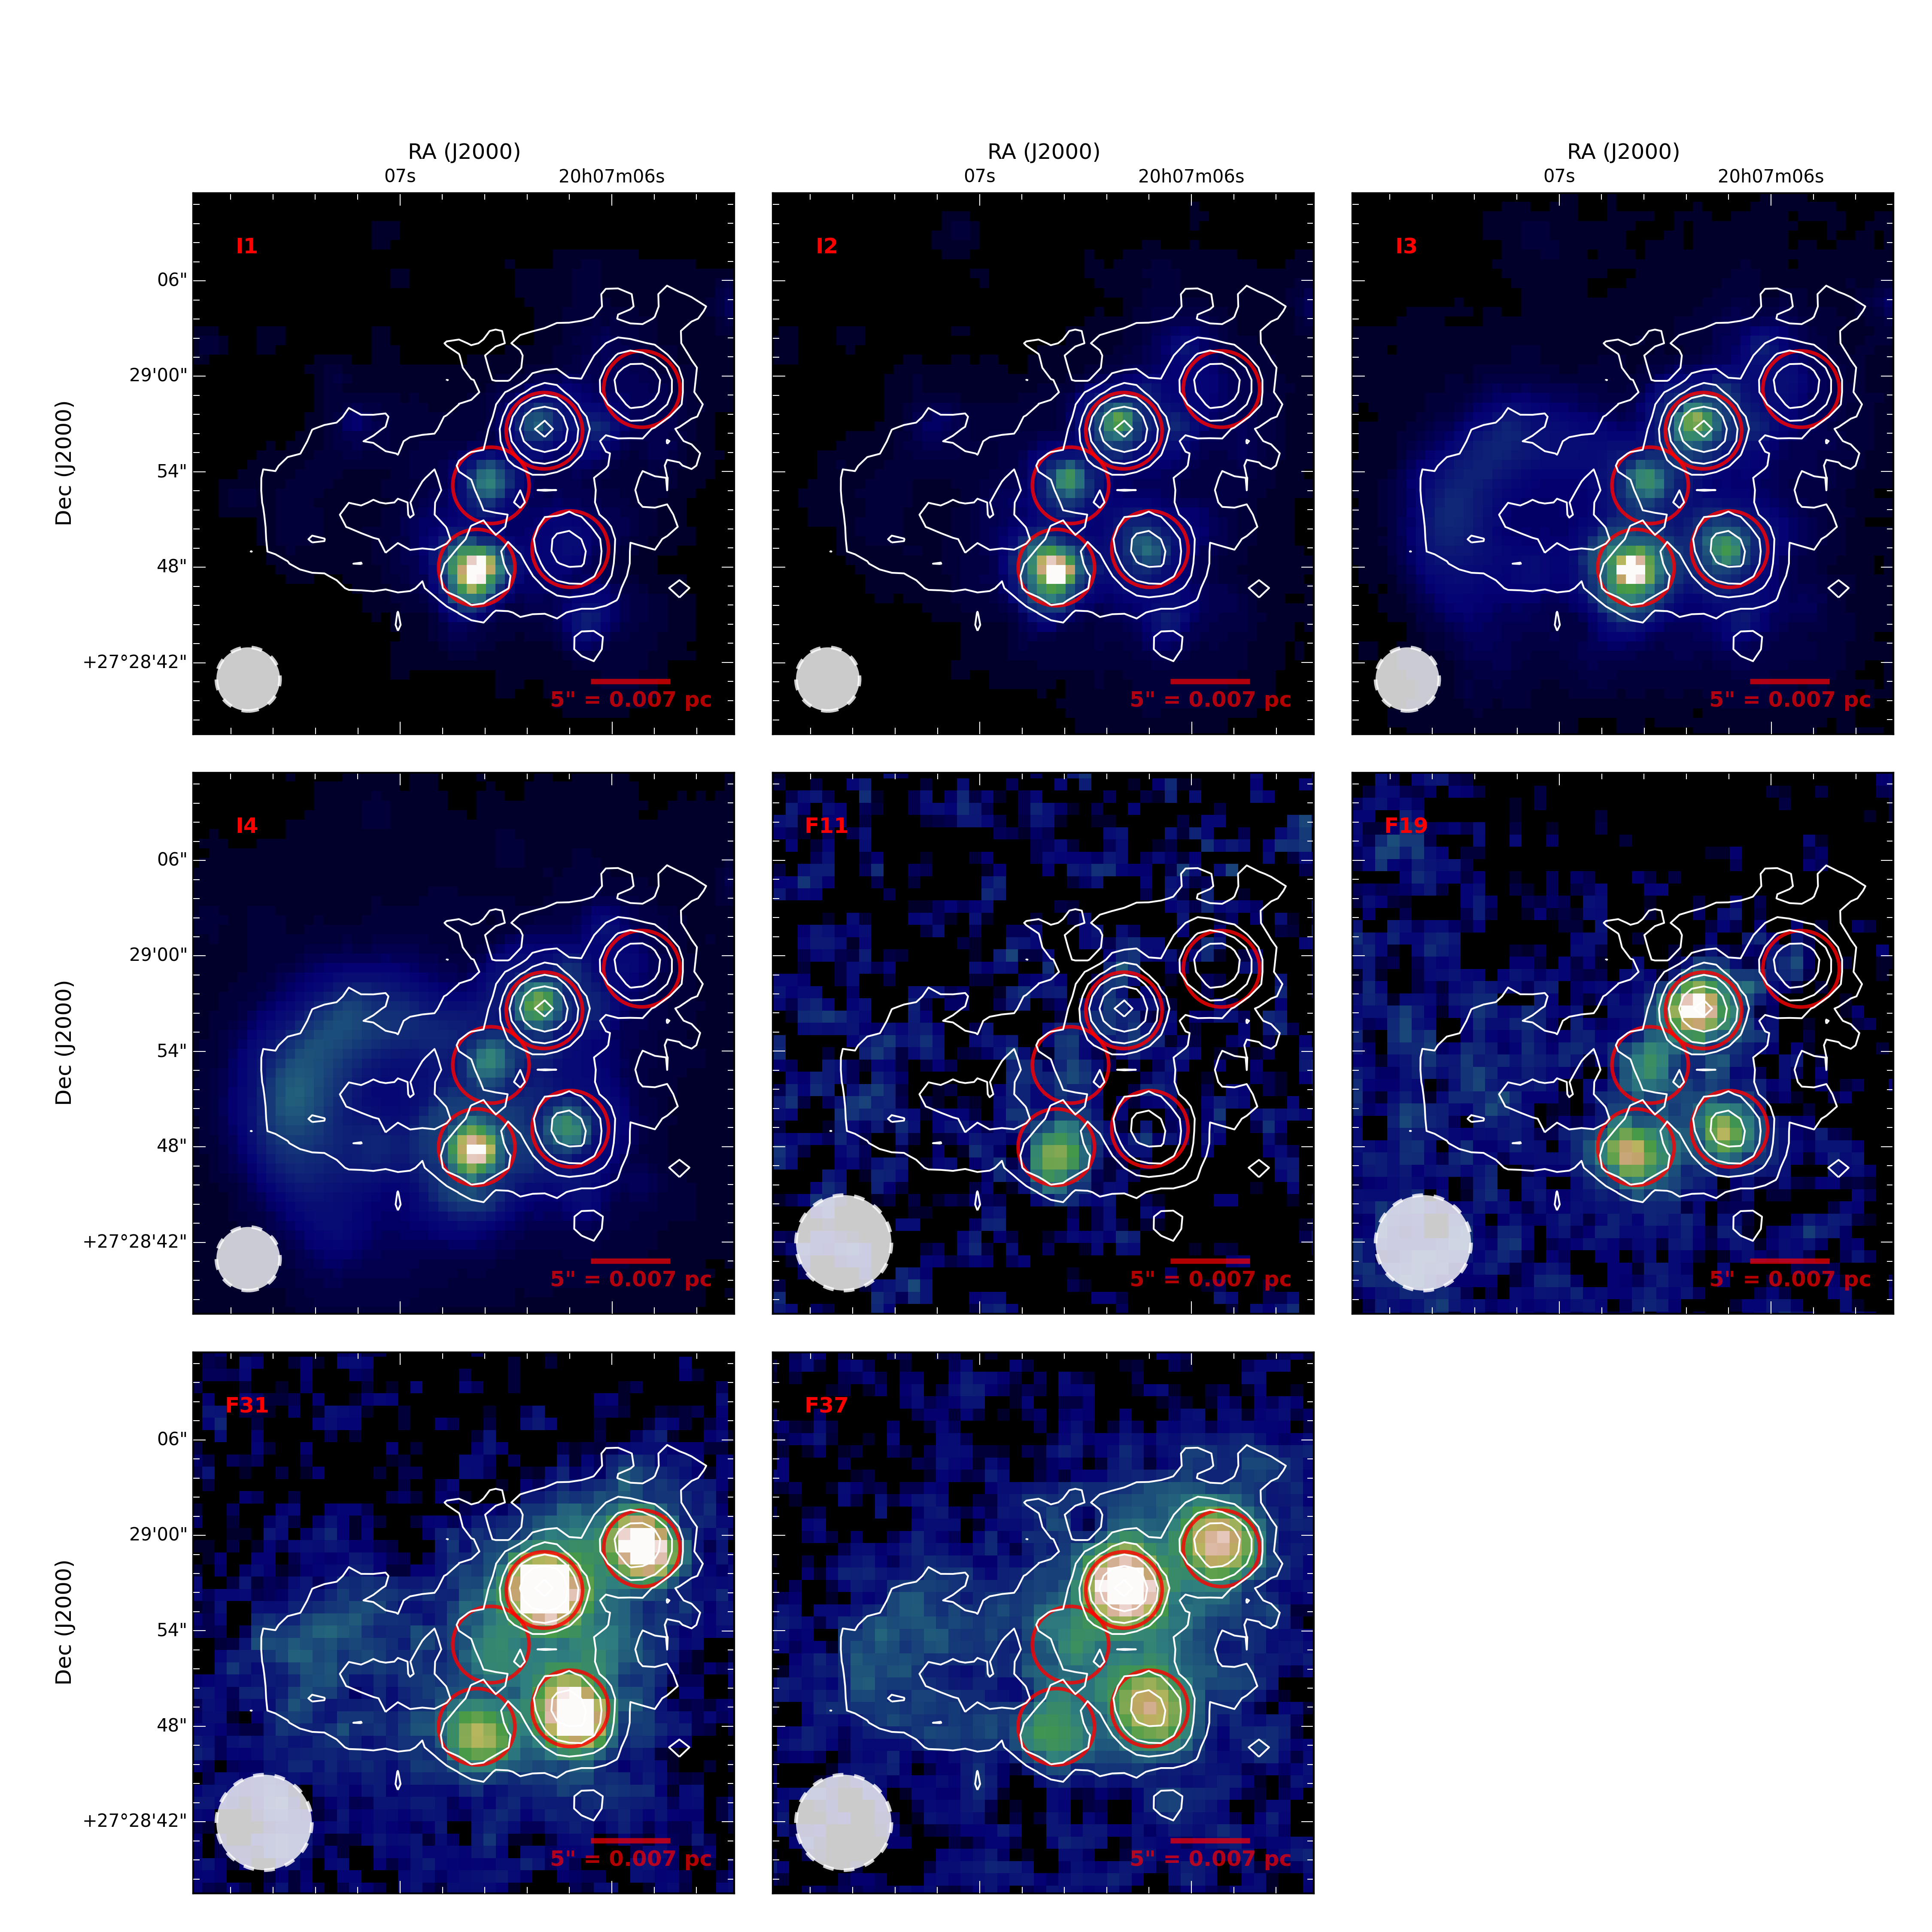
\includegraphics[width=1\textwidth]{Figures/IRAS20050_SOFIA.png}
\label{fig:IRAS20050_mosaic}
\caption{The core of IRAS20050+2720 is seen in the four bands of the \textit{Spitzer} IRAS instrument, as well as with the four FORCAST bands. The increased resolution of FORCAST compared to previous instruments allows to match the long-wavelength emission with its short wavelength counterpart. The stretch in each image is adjusted for optimal readability. The white contours correspond to the FORCAST \SI{37}{\micro\meter} emission [mention the contour levels]. The red circles indicate the location of the five FORCAST point sources in the core.}
\end{center}
\end{figure}

\begin{figure}
\begin{center}
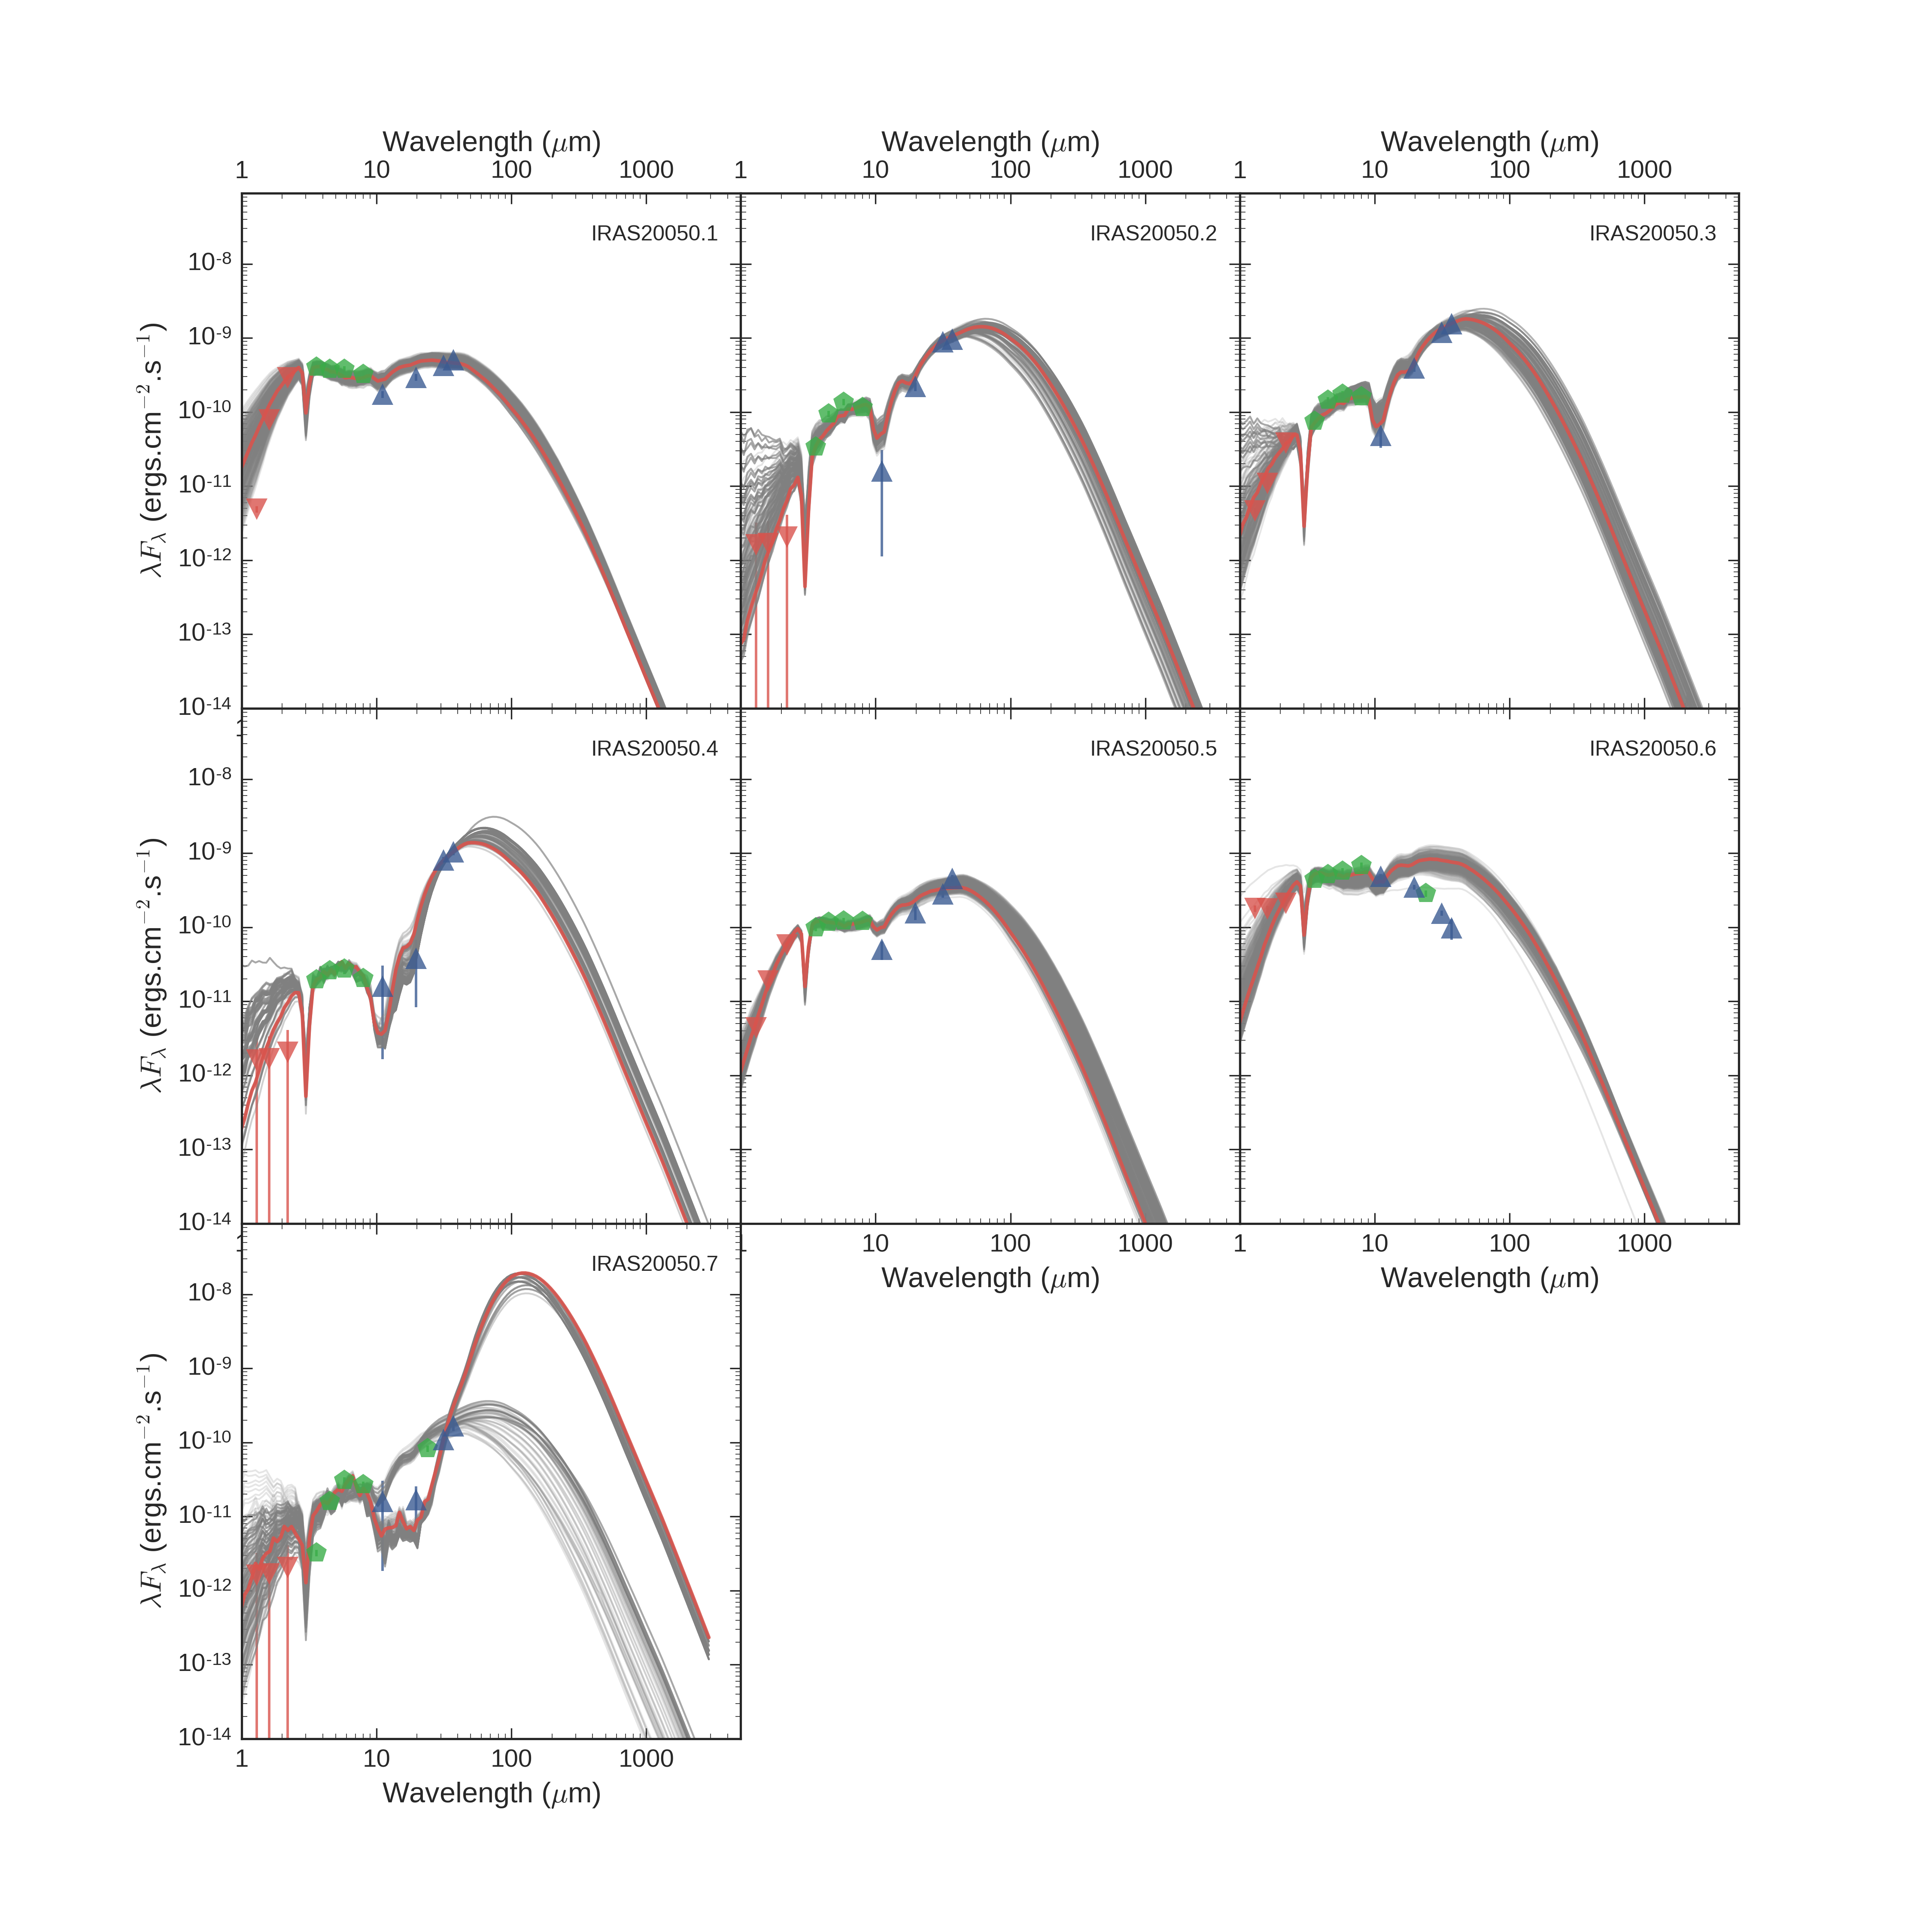
\includegraphics[width=1\textwidth]{Figures/IRAS20050_SEDs.png}
\label{fig:IRAS20050_SEDs}
\caption{}
\end{center}
\end{figure}




\subsection{NGC2071}


\subsubsection{Photometry results and maps}

\begin{figure}
\begin{center}
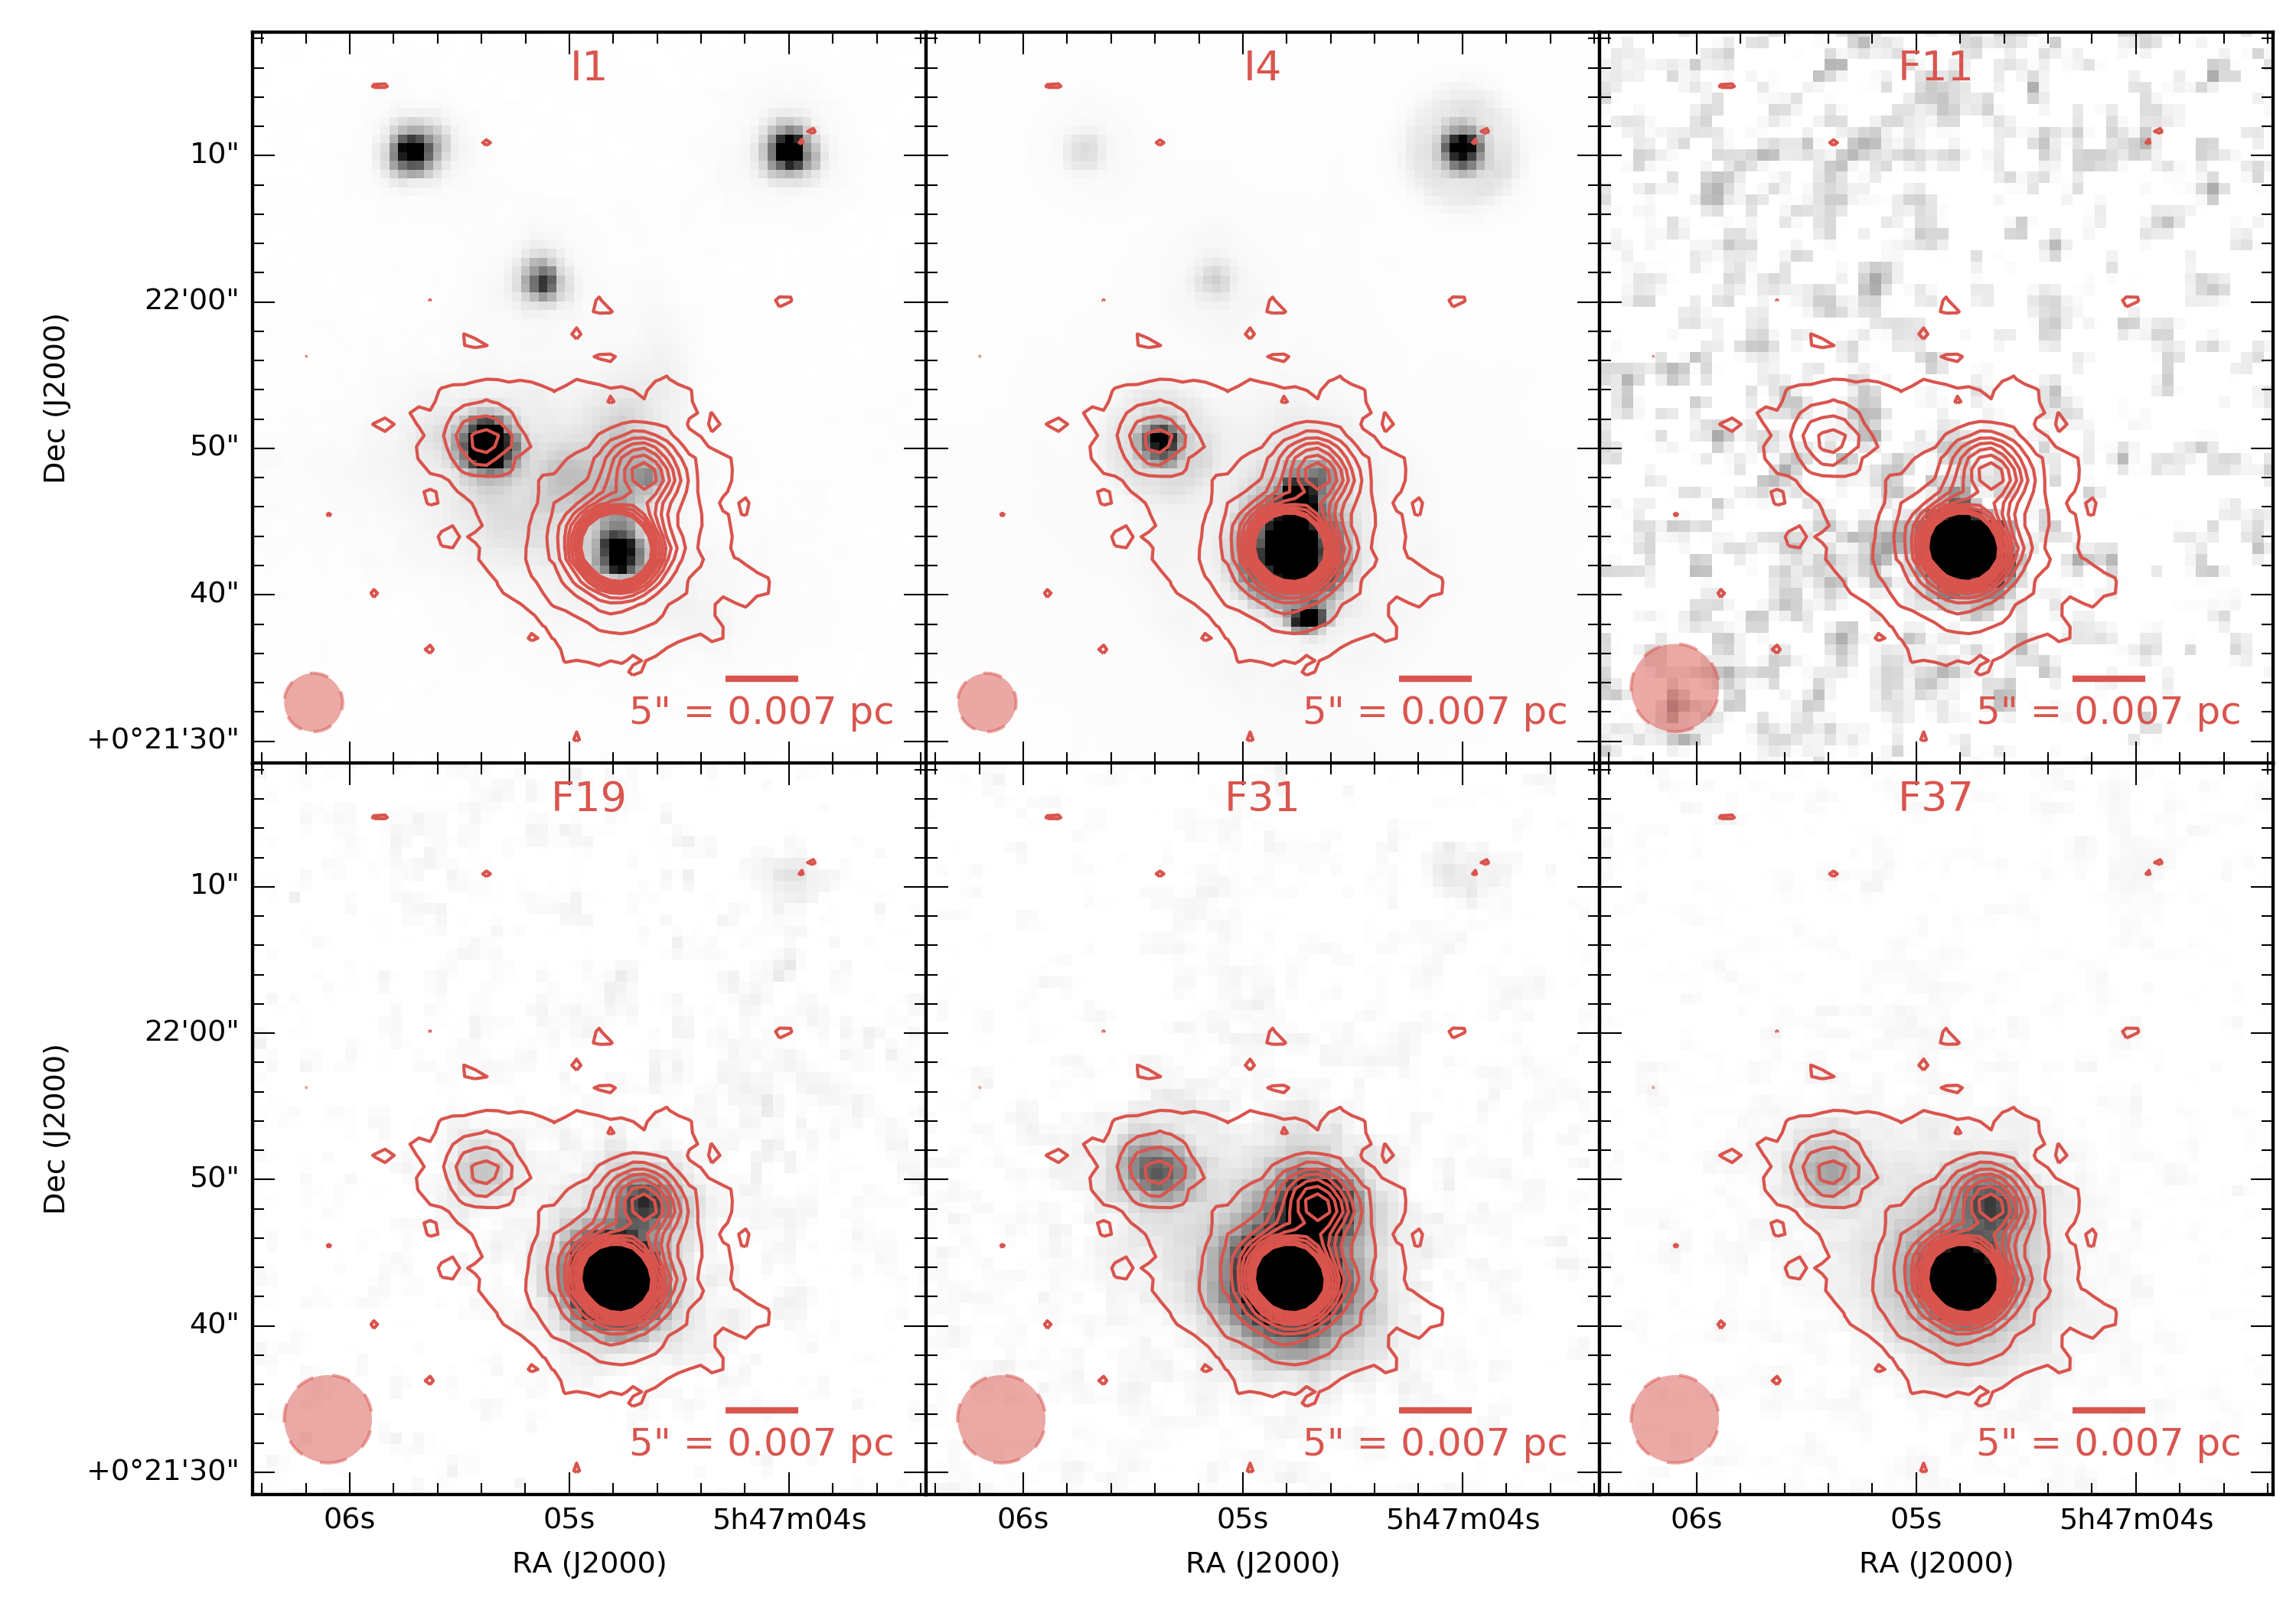
\includegraphics[width=1\textwidth]{Figures/NGC2071_mosaic.png}
\label{fig:NGC2071_mosaic}
\caption{The core of IRAS20050+2720 is seen in the four bands of the \textit{Spitzer} IRAS instrument, as well as with the four FORCAST bands. The increased resolution of FORCAST compared to previous instruments allows to match the long-wavelength emission with its short wavelength counterpart. The stretch in each image is adjusted for optimal readability. The white contours correspond to the FORCAST \SI{37}{\micro\meter} emission [mention the contour levels]. The red circles indicate the location of the five FORCAST point sources in the core.}
\end{center}
\end{figure}

\begin{figure}
\begin{center}
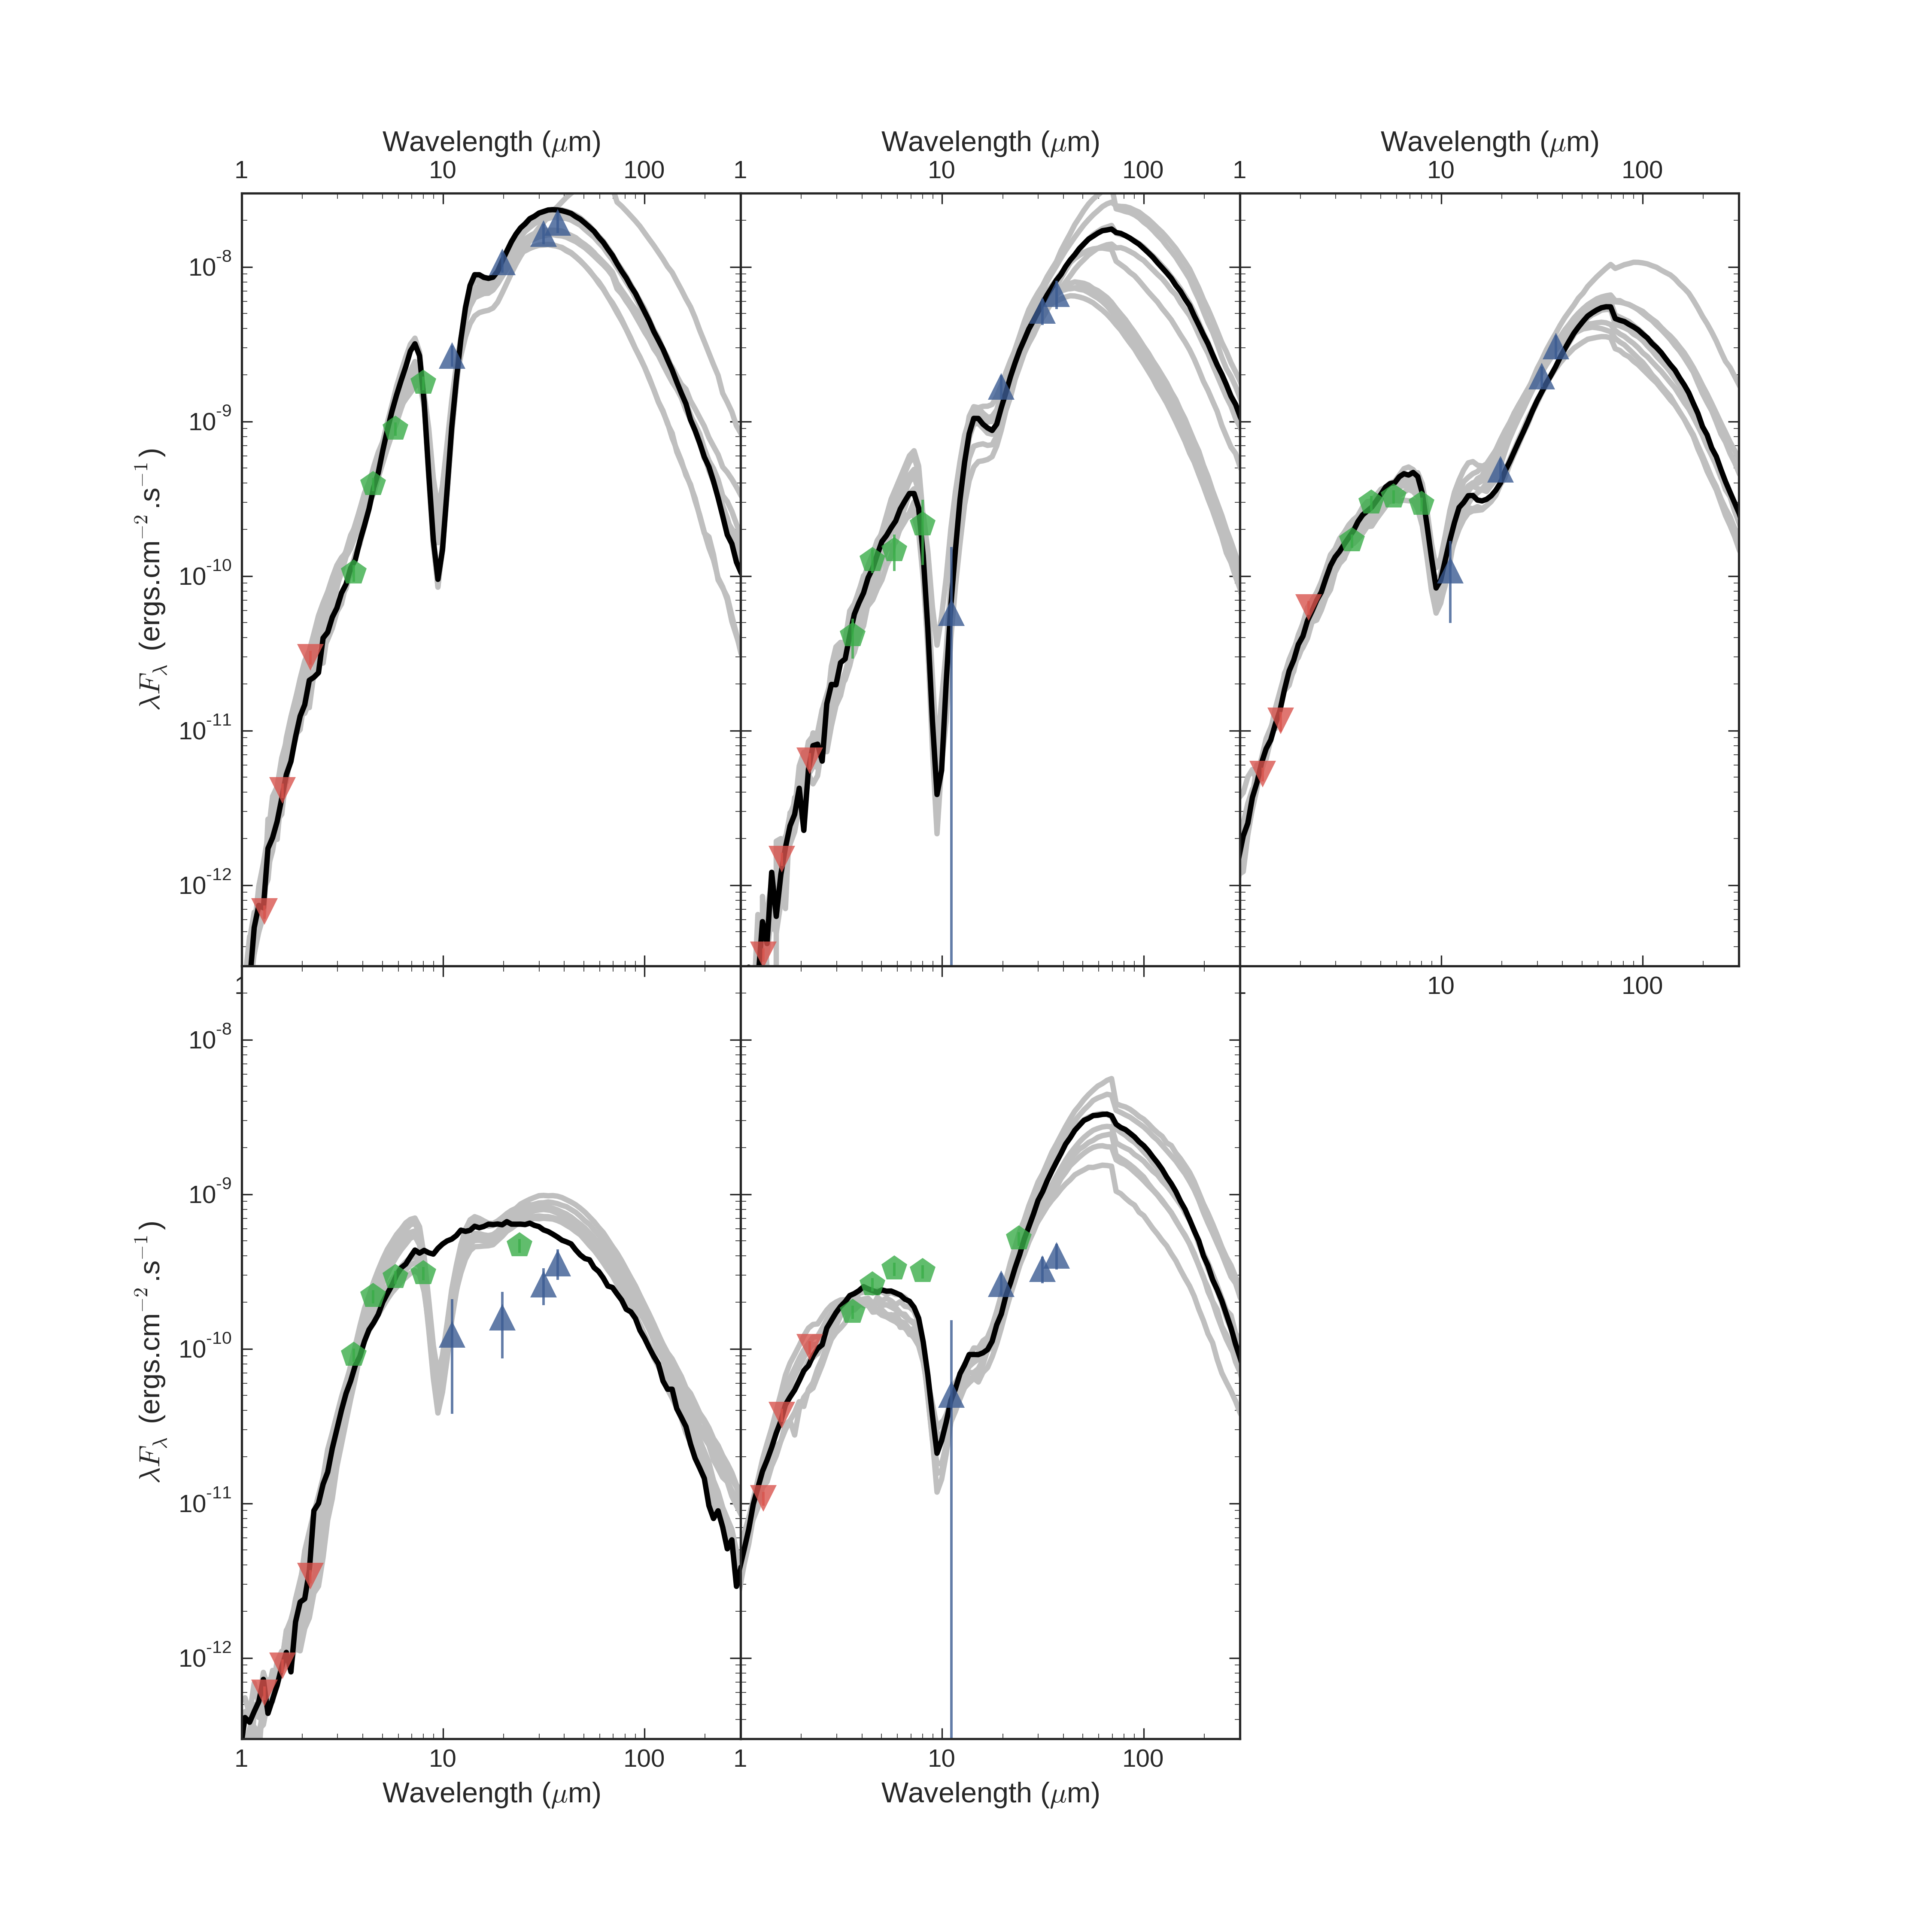
\includegraphics[width=1\textwidth]{Figures/NGC2071_SEDs.png}
\label{fig:NGC2071_SEDs}
\caption{}
\end{center}
\end{figure}

\subsubsection{SEDs}

\subsubsection{Upper limits on other sources in the field}


\subsection{Summary}

Put here the table of photometry + flags



\section{SED and dust modeling}

YE05 assumed the dust opacities of Ossenkopf \& Henning
(1994) appropriate for thin ice mantles after 105 year of coagulation at a gas density of 106 cm-3 (OH5 dust), which several recent studies have shown to be appropriate for cold, dense cores (e.g., Evans et al. 2001; Shirley et al. 2002; Young et al. 2003; Shirley et al. 2005) [LOOK AT REST OF DISCUSSION IN DUNHAM et al. 2010]

\subsection{Radiative transfer models}

We use radiative transfer models to fit the SEDs we observe and extract physical parameters. We explored the tool by \cite{Robitaille:2006cb} as a starting point for this process. While the tool provides results that fit the data well, the large number of parameters makes it difficult to draw meaningful conclusions on the real physics behind the observations. We have observed a large amount of cross-correlations between the model parameters, as well as many local minimas in the $\chi^2$ minimization scheme that is used.

In an effort to understand the dependence of the observations with the physical parameters used in the models, we use the HYPERION radiative transfer code \citep{Robitaille:2011fc} and create our own grid of models by varying a small amount of meaningful parameters. HYPERION is a very versatile code with lots of options for various geometries, but we simplify the problem to its most essential components: a circularly symmetric disk with a power-law envelope.

We explore the various geometries and parameters that are available in the code, and come to following conclusions:
\begin{enumerate}
\item Modeling accretion through an $\alpha$-disk instead of a flared disk is equivalent to increasing the central luminosity by an appropriate amount. Hence, we use only standard flared disks and quote a total central luminosity
\item It is good enough to only vary the total luminosity of the central object, instead of varying its mass, radius and temperature
\item Models are very insensitive to disk mass, when the envelope's mass is larger
\item The model is sensitive to the envelope's mass distribution within a given radius, but not sensitive to the envelope's inner or outer radius
\item The outer radius of the disk has no effect on the models
\item The inner radius of the envelope 
\end{enumerate}

Based on our exploration of HYPERION, we proceed with the following simulation set up. We use a density structure composed of a standard flared disk of \SI{e-3}{\Msun} that extends from the dust sublimation radius out to 50~AU. The scale height at the dust sublimation radius is set to be 10\% of that radius. The disk's flaring power is a constant set to $\beta=1.1$. 

We add an envelope with a central cavity. The envelope extends from 30~AU out to a variable radius, and has a variable mass and power law exponent. The inner cavity has a constant 25 degree opening angle. Setting this latter parameter has some effect that is correlated with the viewing angle.

All elements in our model are using the same dust model by \cite{Draine:2003di}. We have experimented with various other types of dust models, notably with the OH5 dust [REFERENCE], as it was suggested in [CITE TRACY]. We found that the fits with the OH5 dust were much worse. In most cases, it was particularly difficult to fit the \SI{10}{\micro\meter} silicate absorption feature. 

We use a variable foreground extinction also with the same dust model, as we anticipate that most of the extinction along the line of sight will occur in the cluster itself. We chose to not use any ambient medium, as they complicated the interpretation of the results.

We run our simulations using $10^5$ photons, and spherical grids with 199 radial cells, 49 meridional cells, and 1 single azimuthal cell. We have tested these various parameters and sought an optimum of fast computing times and low statistical noise. With this, the calculated uncertainties are a few percent at long wavelengths and can be on the order of 10 to 15 percent at short wavelengths. This is acceptable since the short wavelength range is largely used in the fit to determine the overall external extinction magnitude. At the wavelenghts relevant for the IRAC fluxes, the uncertainties due to the simulation are on the order of 5\% - less than our estimated measurement error. With these parameters, a typical model takes about 5-10 minutes to run on a standard desktop computer. Our wrapper software allows us to run multiple different grids in a row and merge them into one single entity that we can feed to a minimization routine.

In order to fit the data, we use the $\chi^2$ method described in \cite{Robitaille:2007dl}, with the exception of the overall optimal scaling step. We calculate the $\chi^2$ for our targets with all calculated models, inclinations, and a range of values of foreground extinction magnitudes.


%Table of set parameters]

%variable parameters: envelope mass, envelope density power law, source luminosity, inclination, extinction




%This section discusses how we set up a grid of models to fit, and why we moved away from Robitaille's sedfitter. Maybe show some results from the Robitaille's fits?

\subsection{Extracting physical parameters from the fits}
This section discusses the results from the fits: best fits, parameter estimation and variation about the best fits, color-color diagrams, etc.
\begin{itemize}
\item \citep{Shirley:2000gh}: typical masses of protostars are a few tenths to \SI{2}{\Msun}. 

\end{itemize}


\section{Discussion}

\section{Conclusion}
blabla